\documentclass[1p]{elsarticle_modified}
%\bibliographystyle{elsarticle-num}

%\usepackage[colorlinks]{hyperref}
%\usepackage{abbrmath_seonhwa} %\Abb, \Ascr, \Acal ,\Abf, \Afrak
\usepackage{amsfonts}
\usepackage{amssymb}
\usepackage{amsmath}
\usepackage{amsthm}
\usepackage{scalefnt}
\usepackage{amsbsy}
\usepackage{kotex}
\usepackage{caption}
\usepackage{subfig}
\usepackage{color}
\usepackage{graphicx}
\usepackage{xcolor} %% white, black, red, green, blue, cyan, magenta, yellow
\usepackage{float}
\usepackage{setspace}
\usepackage{hyperref}

\usepackage{tikz}
\usetikzlibrary{arrows}

\usepackage{multirow}
\usepackage{array} % fixed length table
\usepackage{hhline}

%%%%%%%%%%%%%%%%%%%%%
\makeatletter
\renewcommand*\env@matrix[1][\arraystretch]{%
	\edef\arraystretch{#1}%
	\hskip -\arraycolsep
	\let\@ifnextchar\new@ifnextchar
	\array{*\c@MaxMatrixCols c}}
\makeatother %https://tex.stackexchange.com/questions/14071/how-can-i-increase-the-line-spacing-in-a-matrix
%%%%%%%%%%%%%%%

\usepackage[normalem]{ulem}

\newcommand{\msout}[1]{\ifmmode\text{\sout{\ensuremath{#1}}}\else\sout{#1}\fi}
%SOURCE: \msout is \stkout macro in https://tex.stackexchange.com/questions/20609/strikeout-in-math-mode

\newcommand{\cancel}[1]{
	\ifmmode
	{\color{red}\msout{#1}}
	\else
	{\color{red}\sout{#1}}
	\fi
}

\newcommand{\add}[1]{
	{\color{blue}\uwave{#1}}
}

\newcommand{\replace}[2]{
	\ifmmode
	{\color{red}\msout{#1}}{\color{blue}\uwave{#2}}
	\else
	{\color{red}\sout{#1}}{\color{blue}\uwave{#2}}
	\fi
}

\newcommand{\Sol}{\mathcal{S}} %segment
\newcommand{\D}{D} %diagram
\newcommand{\A}{\mathcal{A}} %arc


%%%%%%%%%%%%%%%%%%%%%%%%%%%%%5 test

\def\sl{\operatorname{\textup{SL}}(2,\Cbb)}
\def\psl{\operatorname{\textup{PSL}}(2,\Cbb)}
\def\quan{\mkern 1mu \triangleright \mkern 1mu}

\theoremstyle{definition}
\newtheorem{thm}{Theorem}[section]
\newtheorem{prop}[thm]{Proposition}
\newtheorem{lem}[thm]{Lemma}
\newtheorem{ques}[thm]{Question}
\newtheorem{cor}[thm]{Corollary}
\newtheorem{defn}[thm]{Definition}
\newtheorem{exam}[thm]{Example}
\newtheorem{rmk}[thm]{Remark}
\newtheorem{alg}[thm]{Algorithm}

\newcommand{\I}{\sqrt{-1}}
\begin{document}

%\begin{frontmatter}
%
%\title{Boundary parabolic representations of knots up to 8 crossings}
%
%%% Group authors per affiliation:
%\author{Yunhi Cho} 
%\address{Department of Mathematics, University of Seoul, Seoul, Korea}
%\ead{yhcho@uos.ac.kr}
%
%
%\author{Seonhwa Kim} %\fnref{s_kim}}
%\address{Center for Geometry and Physics, Institute for Basic Science, Pohang, 37673, Korea}
%\ead{ryeona17@ibs.re.kr}
%
%\author{Hyuk Kim}
%\address{Department of Mathematical Sciences, Seoul National University, Seoul 08826, Korea}
%\ead{hyukkim@snu.ac.kr}
%
%\author{Seokbeom Yoon}
%\address{Department of Mathematical Sciences, Seoul National University, Seoul, 08826,  Korea}
%\ead{sbyoon15@snu.ac.kr}
%
%\begin{abstract}
%We find all boundary parabolic representation of knots up to 8 crossings.
%
%\end{abstract}
%\begin{keyword}
%    \MSC[2010] 57M25 
%\end{keyword}
%
%\end{frontmatter}

%\linenumbers
%\tableofcontents
%
\newcommand\colored[1]{\textcolor{white}{\rule[-0.35ex]{0.8em}{1.4ex}}\kern-0.8em\color{red} #1}%
%\newcommand\colored[1]{\textcolor{white}{ #1}\kern-2.17ex	\textcolor{white}{ #1}\kern-1.81ex	\textcolor{white}{ #1}\kern-2.15ex\color{red}#1	}

{\Large $\underline{12a_{0922}~(K12a_{0922})}$}

\setlength{\tabcolsep}{10pt}
\renewcommand{\arraystretch}{1.6}
\vspace{1cm}\begin{tabular}{m{100pt}>{\centering\arraybackslash}m{274pt}}
\multirow{5}{120pt}{
	\centering
	\includegraphics[width=112pt]{../../../GIT/diagram.site/Diagrams/png/1723_12a_0922.png}\\
\ \ \ A knot diagram\footnotemark}&
\allowdisplaybreaks
\textbf{Linearized knot diagam} \\
\cline{2-2}
 &
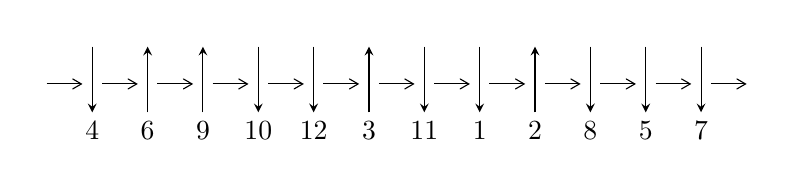
\begin{tikzpicture}[x=20pt, y=17pt]
	% nodes
	\node (C0) at (0, 0) {};
	\node (C1) at (1, 0) {};
	\node (C1U) at (1, +1) {};
	\node (C1D) at (1, -1) {4};

	\node (C2) at (2, 0) {};
	\node (C2U) at (2, +1) {};
	\node (C2D) at (2, -1) {6};

	\node (C3) at (3, 0) {};
	\node (C3U) at (3, +1) {};
	\node (C3D) at (3, -1) {9};

	\node (C4) at (4, 0) {};
	\node (C4U) at (4, +1) {};
	\node (C4D) at (4, -1) {10};

	\node (C5) at (5, 0) {};
	\node (C5U) at (5, +1) {};
	\node (C5D) at (5, -1) {12};

	\node (C6) at (6, 0) {};
	\node (C6U) at (6, +1) {};
	\node (C6D) at (6, -1) {3};

	\node (C7) at (7, 0) {};
	\node (C7U) at (7, +1) {};
	\node (C7D) at (7, -1) {11};

	\node (C8) at (8, 0) {};
	\node (C8U) at (8, +1) {};
	\node (C8D) at (8, -1) {1};

	\node (C9) at (9, 0) {};
	\node (C9U) at (9, +1) {};
	\node (C9D) at (9, -1) {2};

	\node (C10) at (10, 0) {};
	\node (C10U) at (10, +1) {};
	\node (C10D) at (10, -1) {8};

	\node (C11) at (11, 0) {};
	\node (C11U) at (11, +1) {};
	\node (C11D) at (11, -1) {5};

	\node (C12) at (12, 0) {};
	\node (C12U) at (12, +1) {};
	\node (C12D) at (12, -1) {7};
	\node (C13) at (13, 0) {};

	% arrows
	\draw[->,>={angle 60}]
	(C0) edge (C1) (C1) edge (C2) (C2) edge (C3) (C3) edge (C4) (C4) edge (C5) (C5) edge (C6) (C6) edge (C7) (C7) edge (C8) (C8) edge (C9) (C9) edge (C10) (C10) edge (C11) (C11) edge (C12) (C12) edge (C13) ;	\draw[->,>=stealth]
	(C1U) edge (C1D) (C2D) edge (C2U) (C3D) edge (C3U) (C4U) edge (C4D) (C5U) edge (C5D) (C6D) edge (C6U) (C7U) edge (C7D) (C8U) edge (C8D) (C9D) edge (C9U) (C10U) edge (C10D) (C11U) edge (C11D) (C12U) edge (C12D) ;
	\end{tikzpicture} \\
\hhline{~~} \\& 
\textbf{Solving Sequence} \\ \cline{2-2} 
 &
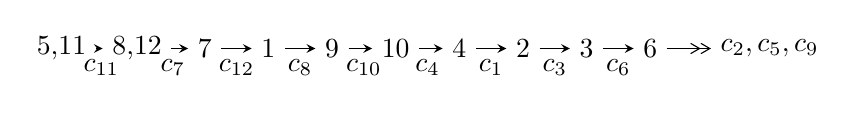
\begin{tikzpicture}[x=23pt, y=7pt]
	% node
	\node (A0) at (-1/8, 0) {5,11};
	\node (A1) at (17/16, 0) {8,12};
	\node (A2) at (17/8, 0) {7};
	\node (A3) at (25/8, 0) {1};
	\node (A4) at (33/8, 0) {9};
	\node (A5) at (41/8, 0) {10};
	\node (A6) at (49/8, 0) {4};
	\node (A7) at (57/8, 0) {2};
	\node (A8) at (65/8, 0) {3};
	\node (A9) at (73/8, 0) {6};
	\node (C1) at (1/2, -1) {$c_{11}$};
	\node (C2) at (13/8, -1) {$c_{7}$};
	\node (C3) at (21/8, -1) {$c_{12}$};
	\node (C4) at (29/8, -1) {$c_{8}$};
	\node (C5) at (37/8, -1) {$c_{10}$};
	\node (C6) at (45/8, -1) {$c_{4}$};
	\node (C7) at (53/8, -1) {$c_{1}$};
	\node (C8) at (61/8, -1) {$c_{3}$};
	\node (C9) at (69/8, -1) {$c_{6}$};
	\node (A10) at (11, 0) {$c_{2},c_{5},c_{9}$};

	% edge
	\draw[->,>=stealth]	
	(A0) edge (A1) (A1) edge (A2) (A2) edge (A3) (A3) edge (A4) (A4) edge (A5) (A5) edge (A6) (A6) edge (A7) (A7) edge (A8) (A8) edge (A9) ;
	\draw[->>,>={angle 60}]	
	(A9) edge (A10);
\end{tikzpicture} \\ 

\end{tabular} \\

\footnotetext{
The image of knot diagram is generated by the software ``\textbf{Draw programme}" developed by Andrew Bartholomew(\url{http://www.layer8.co.uk/maths/draw/index.htm\#Running-draw}), where we modified some parts for our purpose(\url{https://github.com/CATsTAILs/LinksPainter}).
}\phantom \\ \newline 
\centering \textbf{Ideals for irreducible components\footnotemark of $X_{\text{par}}$} 
 
\begin{align*}
I^u_{1}&=\langle 
-4.33030\times10^{1482} u^{197}-8.31840\times10^{1482} u^{196}+\cdots+5.08986\times10^{1483} b-3.67386\times10^{1487},\\
\phantom{I^u_{1}}&\phantom{= \langle  }6.23201\times10^{1487} u^{197}+1.16404\times10^{1488} u^{196}+\cdots+4.53166\times10^{1488} a+6.49088\times10^{1492},\\
\phantom{I^u_{1}}&\phantom{= \langle  }u^{198}+u^{197}+\cdots-1502406 u-89033\rangle \\
I^u_{2}&=\langle 
-7.38108\times10^{78} u^{56}+2.03170\times10^{79} u^{55}+\cdots+4.01238\times10^{78} b-4.19152\times10^{78},\\
\phantom{I^u_{2}}&\phantom{= \langle  }-4.91319\times10^{78} u^{56}+1.93609\times10^{79} u^{55}+\cdots+4.01238\times10^{78} a+3.19386\times10^{78},\;u^{57}-2 u^{56}+\cdots+7 u-1\rangle \\
\\
\end{align*}
\raggedright * 2 irreducible components of $\dim_{\mathbb{C}}=0$, with total 255 representations.\\
\footnotetext{All coefficients of polynomials are rational numbers. But the coefficients are sometimes approximated in decimal forms when there is not enough margin.}
\newpage
\renewcommand{\arraystretch}{1}
\centering \section*{I. $I^u_{1}= \langle -4.33\times10^{1482} u^{197}-8.32\times10^{1482} u^{196}+\cdots+5.09\times10^{1483} b-3.67\times10^{1487},\;6.23\times10^{1487} u^{197}+1.16\times10^{1488} u^{196}+\cdots+4.53\times10^{1488} a+6.49\times10^{1492},\;u^{198}+u^{197}+\cdots-1502406 u-89033 \rangle$}
\flushleft \textbf{(i) Arc colorings}\\
\begin{tabular}{m{7pt} m{180pt} m{7pt} m{180pt} }
\flushright $a_{5}=$&$\begin{pmatrix}0\\u\end{pmatrix}$ \\
\flushright $a_{11}=$&$\begin{pmatrix}1\\0\end{pmatrix}$ \\
\flushright $a_{8}=$&$\begin{pmatrix}-0.137522 u^{197}-0.256868 u^{196}+\cdots-257540. u-14323.4\\0.0850769 u^{197}+0.163431 u^{196}+\cdots+129633. u+7218.00\end{pmatrix}$ \\
\flushright $a_{12}=$&$\begin{pmatrix}1\\u^2\end{pmatrix}$ \\
\flushright $a_{7}=$&$\begin{pmatrix}-0.0524447 u^{197}-0.0934372 u^{196}+\cdots-127907. u-7105.41\\0.0850769 u^{197}+0.163431 u^{196}+\cdots+129633. u+7218.00\end{pmatrix}$ \\
\flushright $a_{1}=$&$\begin{pmatrix}0.110451 u^{197}+0.206797 u^{196}+\cdots+174835. u+9688.16\\-0.0186996 u^{197}-0.0351781 u^{196}+\cdots-26798.6 u-1481.48\end{pmatrix}$ \\
\flushright $a_{9}=$&$\begin{pmatrix}0.0836670 u^{197}+0.176503 u^{196}+\cdots+142987. u+8077.11\\0.0528392 u^{197}+0.100875 u^{196}+\cdots+93354.4 u+5195.69\end{pmatrix}$ \\
\flushright $a_{10}=$&$\begin{pmatrix}-0.0121678 u^{197}-0.0236557 u^{196}+\cdots-18829.4 u-1038.53\\0.0507746 u^{197}+0.0932345 u^{196}+\cdots+76768.4 u+4239.01\end{pmatrix}$ \\
\flushright $a_{4}=$&$\begin{pmatrix}0.0597915 u^{197}+0.116686 u^{196}+\cdots+108658. u+6080.30\\-0.0628572 u^{197}-0.119933 u^{196}+\cdots-104786. u-5835.55\end{pmatrix}$ \\
\flushright $a_{2}=$&$\begin{pmatrix}0.116474 u^{197}+0.235488 u^{196}+\cdots+199053. u+11195.1\\0.0673832 u^{197}+0.121228 u^{196}+\cdots+126606. u+7001.79\end{pmatrix}$ \\
\flushright $a_{3}=$&$\begin{pmatrix}-0.172309 u^{197}-0.339160 u^{196}+\cdots-303862. u-17016.3\\-0.0514320 u^{197}-0.0902693 u^{196}+\cdots-98636.6 u-5439.58\end{pmatrix}$ \\
\flushright $a_{6}=$&$\begin{pmatrix}- u\\- u^3+u\end{pmatrix}$\\&\end{tabular}
\flushleft \textbf{(ii) Obstruction class $= -1$}\\~\\
\flushleft \textbf{(iii) Cusp Shapes $= -0.316742 u^{197}-0.593665 u^{196}+\cdots-519214. u-28823.3$}\\~\\
\newpage\renewcommand{\arraystretch}{1}
\flushleft \textbf{(iv) u-Polynomials at the component}\newline \\
\begin{tabular}{m{50pt}|m{274pt}}
Crossings & \hspace{64pt}u-Polynomials at each crossing \\
\hline $$\begin{aligned}c_{1}\end{aligned}$$&$\begin{aligned}
&u^{198}-13 u^{197}+\cdots-79 u+47
\end{aligned}$\\
\hline $$\begin{aligned}c_{2},c_{6}\end{aligned}$$&$\begin{aligned}
&u^{198}-44 u^{196}+\cdots+4 u-1
\end{aligned}$\\
\hline $$\begin{aligned}c_{3}\end{aligned}$$&$\begin{aligned}
&u^{198}-2 u^{197}+\cdots-317 u-23
\end{aligned}$\\
\hline $$\begin{aligned}c_{4}\end{aligned}$$&$\begin{aligned}
&u^{198}-32 u^{196}+\cdots+16388029166 u-6212469373
\end{aligned}$\\
\hline $$\begin{aligned}c_{5},c_{11}\end{aligned}$$&$\begin{aligned}
&u^{198}+u^{197}+\cdots-1502406 u-89033
\end{aligned}$\\
\hline $$\begin{aligned}c_{7},c_{10}\end{aligned}$$&$\begin{aligned}
&u^{198}+15 u^{197}+\cdots-46454 u+12173
\end{aligned}$\\
\hline $$\begin{aligned}c_{8}\end{aligned}$$&$\begin{aligned}
&u^{198}-7 u^{196}+\cdots-6925 u-181
\end{aligned}$\\
\hline $$\begin{aligned}c_{9}\end{aligned}$$&$\begin{aligned}
&u^{198}+3 u^{197}+\cdots+18797 u-3181
\end{aligned}$\\
\hline $$\begin{aligned}c_{12}\end{aligned}$$&$\begin{aligned}
&u^{198}-12 u^{196}+\cdots-4308718 u-110767
\end{aligned}$\\
\hline
\end{tabular}\\~\\
\newpage\renewcommand{\arraystretch}{1}
\flushleft \textbf{(v) Riley Polynomials at the component}\newline \\
\begin{tabular}{m{50pt}|m{274pt}}
Crossings & \hspace{64pt}Riley Polynomials at each crossing \\
\hline $$\begin{aligned}c_{1}\end{aligned}$$&$\begin{aligned}
&y^{198}-9 y^{197}+\cdots-185029 y+2209
\end{aligned}$\\
\hline $$\begin{aligned}c_{2},c_{6}\end{aligned}$$&$\begin{aligned}
&y^{198}-88 y^{197}+\cdots-48 y+1
\end{aligned}$\\
\hline $$\begin{aligned}c_{3}\end{aligned}$$&$\begin{aligned}
&y^{198}+28 y^{197}+\cdots+36775 y+529
\end{aligned}$\\
\hline $$\begin{aligned}c_{4}\end{aligned}$$&$\begin{aligned}
&y^{198}-64 y^{197}+\cdots-7.98\times10^{20} y+3.86\times10^{19}
\end{aligned}$\\
\hline $$\begin{aligned}c_{5},c_{11}\end{aligned}$$&$\begin{aligned}
&y^{198}-119 y^{197}+\cdots+2069262907500 y+7926875089
\end{aligned}$\\
\hline $$\begin{aligned}c_{7},c_{10}\end{aligned}$$&$\begin{aligned}
&y^{198}+107 y^{197}+\cdots+8292010772 y+148181929
\end{aligned}$\\
\hline $$\begin{aligned}c_{8}\end{aligned}$$&$\begin{aligned}
&y^{198}-14 y^{197}+\cdots-8988859 y+32761
\end{aligned}$\\
\hline $$\begin{aligned}c_{9}\end{aligned}$$&$\begin{aligned}
&y^{198}+47 y^{197}+\cdots+695194011 y+10118761
\end{aligned}$\\
\hline $$\begin{aligned}c_{12}\end{aligned}$$&$\begin{aligned}
&y^{198}-24 y^{197}+\cdots-172765777322 y+12269328289
\end{aligned}$\\
\hline
\end{tabular}\\~\\
\newpage\flushleft \textbf{(vi) Complex Volumes and Cusp Shapes}
$$\begin{array}{c|c|c}  
\text{Solutions to }I^u_{1}& \I (\text{vol} + \sqrt{-1}CS) & \text{Cusp shape}\\
 \hline 
\begin{aligned}
u &= \phantom{-}0.979597 + 0.260723 I \\
a &= -0.189061 + 0.971484 I \\
b &= \phantom{-}0.23238 - 1.78984 I\end{aligned}
 & \phantom{-}2.35768 - 8.58224 I & \phantom{-0.000000 } 0 \\ \hline\begin{aligned}
u &= \phantom{-}0.979597 - 0.260723 I \\
a &= -0.189061 - 0.971484 I \\
b &= \phantom{-}0.23238 + 1.78984 I\end{aligned}
 & \phantom{-}2.35768 + 8.58224 I & \phantom{-0.000000 } 0 \\ \hline\begin{aligned}
u &= -0.976264 + 0.289248 I \\
a &= \phantom{-}1.052900 + 0.583265 I \\
b &= \phantom{-}0.310457 - 1.237310 I\end{aligned}
 & \phantom{-}0.881847 + 0.059937 I & \phantom{-0.000000 } 0 \\ \hline\begin{aligned}
u &= -0.976264 - 0.289248 I \\
a &= \phantom{-}1.052900 - 0.583265 I \\
b &= \phantom{-}0.310457 + 1.237310 I\end{aligned}
 & \phantom{-}0.881847 - 0.059937 I & \phantom{-0.000000 } 0 \\ \hline\begin{aligned}
u &= \phantom{-}1.020100 + 0.034531 I \\
a &= -0.319655 + 0.225581 I \\
b &= -2.15211 + 0.01386 I\end{aligned}
 & -7.61481 - 0.13040 I & \phantom{-0.000000 } 0 \\ \hline\begin{aligned}
u &= \phantom{-}1.020100 - 0.034531 I \\
a &= -0.319655 - 0.225581 I \\
b &= -2.15211 - 0.01386 I\end{aligned}
 & -7.61481 + 0.13040 I & \phantom{-0.000000 } 0 \\ \hline\begin{aligned}
u &= \phantom{-}0.263199 + 0.926297 I \\
a &= \phantom{-}0.80177 + 1.49507 I \\
b &= -0.207876 - 1.091400 I\end{aligned}
 & \phantom{-}3.95365 - 0.06681 I & \phantom{-0.000000 } 0 \\ \hline\begin{aligned}
u &= \phantom{-}0.263199 - 0.926297 I \\
a &= \phantom{-}0.80177 - 1.49507 I \\
b &= -0.207876 + 1.091400 I\end{aligned}
 & \phantom{-}3.95365 + 0.06681 I & \phantom{-0.000000 } 0 \\ \hline\begin{aligned}
u &= -0.927670 + 0.242740 I \\
a &= -1.56795 + 0.56102 I \\
b &= -0.379394 + 1.076750 I\end{aligned}
 & \phantom{-}3.82507 + 2.32250 I & \phantom{-0.000000 } 0 \\ \hline\begin{aligned}
u &= -0.927670 - 0.242740 I \\
a &= -1.56795 - 0.56102 I \\
b &= -0.379394 - 1.076750 I\end{aligned}
 & \phantom{-}3.82507 - 2.32250 I & \phantom{-0.000000 } 0\\
 \hline 
 \end{array}$$\newpage$$\begin{array}{c|c|c}  
\text{Solutions to }I^u_{1}& \I (\text{vol} + \sqrt{-1}CS) & \text{Cusp shape}\\
 \hline 
\begin{aligned}
u &= -0.501779 + 0.913475 I \\
a &= \phantom{-}0.782654 + 0.425143 I \\
b &= -0.802456 - 0.357086 I\end{aligned}
 & -0.59594 - 2.49768 I & \phantom{-0.000000 } 0 \\ \hline\begin{aligned}
u &= -0.501779 - 0.913475 I \\
a &= \phantom{-}0.782654 - 0.425143 I \\
b &= -0.802456 + 0.357086 I\end{aligned}
 & -0.59594 + 2.49768 I & \phantom{-0.000000 } 0 \\ \hline\begin{aligned}
u &= -0.047048 + 1.049100 I \\
a &= \phantom{-}0.49318 - 1.79961 I \\
b &= -0.501460 + 1.063930 I\end{aligned}
 & \phantom{-}1.42910 + 2.33740 I & \phantom{-0.000000 } 0 \\ \hline\begin{aligned}
u &= -0.047048 - 1.049100 I \\
a &= \phantom{-}0.49318 + 1.79961 I \\
b &= -0.501460 - 1.063930 I\end{aligned}
 & \phantom{-}1.42910 - 2.33740 I & \phantom{-0.000000 } 0 \\ \hline\begin{aligned}
u &= -0.938760 + 0.132915 I \\
a &= -1.65662 + 0.75214 I \\
b &= -0.565123 - 0.938852 I\end{aligned}
 & -1.06331 + 2.15989 I & \phantom{-0.000000 } 0 \\ \hline\begin{aligned}
u &= -0.938760 - 0.132915 I \\
a &= -1.65662 - 0.75214 I \\
b &= -0.565123 + 0.938852 I\end{aligned}
 & -1.06331 - 2.15989 I & \phantom{-0.000000 } 0 \\ \hline\begin{aligned}
u &= \phantom{-}0.815697 + 0.464782 I \\
a &= \phantom{-}0.392530 + 0.686869 I \\
b &= \phantom{-}0.151914 - 1.052260 I\end{aligned}
 & \phantom{-}2.32733 - 5.14885 I & \phantom{-0.000000 } 0 \\ \hline\begin{aligned}
u &= \phantom{-}0.815697 - 0.464782 I \\
a &= \phantom{-}0.392530 - 0.686869 I \\
b &= \phantom{-}0.151914 + 1.052260 I\end{aligned}
 & \phantom{-}2.32733 + 5.14885 I & \phantom{-0.000000 } 0 \\ \hline\begin{aligned}
u &= -1.007520 + 0.342004 I \\
a &= -0.613795 - 0.604715 I \\
b &= -0.83829 + 1.17462 I\end{aligned}
 & \phantom{-}0.36079 + 3.51595 I & \phantom{-0.000000 } 0 \\ \hline\begin{aligned}
u &= -1.007520 - 0.342004 I \\
a &= -0.613795 + 0.604715 I \\
b &= -0.83829 - 1.17462 I\end{aligned}
 & \phantom{-}0.36079 - 3.51595 I & \phantom{-0.000000 } 0\\
 \hline 
 \end{array}$$\newpage$$\begin{array}{c|c|c}  
\text{Solutions to }I^u_{1}& \I (\text{vol} + \sqrt{-1}CS) & \text{Cusp shape}\\
 \hline 
\begin{aligned}
u &= \phantom{-}0.927398 + 0.088914 I \\
a &= \phantom{-}1.37670 - 1.77368 I \\
b &= \phantom{-}0.381932 + 0.901393 I\end{aligned}
 & -3.72888 + 2.13591 I & \phantom{-0.000000 } 0 \\ \hline\begin{aligned}
u &= \phantom{-}0.927398 - 0.088914 I \\
a &= \phantom{-}1.37670 + 1.77368 I \\
b &= \phantom{-}0.381932 - 0.901393 I\end{aligned}
 & -3.72888 - 2.13591 I & \phantom{-0.000000 } 0 \\ \hline\begin{aligned}
u &= -0.168521 + 1.056970 I \\
a &= -0.46516 - 1.41329 I \\
b &= \phantom{-}0.495151 + 1.182070 I\end{aligned}
 & \phantom{-}0.08704 - 8.95349 I & \phantom{-0.000000 } 0 \\ \hline\begin{aligned}
u &= -0.168521 - 1.056970 I \\
a &= -0.46516 + 1.41329 I \\
b &= \phantom{-}0.495151 - 1.182070 I\end{aligned}
 & \phantom{-}0.08704 + 8.95349 I & \phantom{-0.000000 } 0 \\ \hline\begin{aligned}
u &= \phantom{-}0.923379 + 0.072047 I \\
a &= -1.18541 + 0.92189 I \\
b &= -0.780980 - 1.026960 I\end{aligned}
 & -3.66143 - 3.37349 I & \phantom{-0.000000 } 0 \\ \hline\begin{aligned}
u &= \phantom{-}0.923379 - 0.072047 I \\
a &= -1.18541 - 0.92189 I \\
b &= -0.780980 + 1.026960 I\end{aligned}
 & -3.66143 + 3.37349 I & \phantom{-0.000000 } 0 \\ \hline\begin{aligned}
u &= -0.896238 + 0.183671 I \\
a &= \phantom{-}0.03102 + 2.02801 I \\
b &= -0.21018 - 1.43390 I\end{aligned}
 & \phantom{-}4.04748 - 0.45155 I & \phantom{-0.000000 } 0 \\ \hline\begin{aligned}
u &= -0.896238 - 0.183671 I \\
a &= \phantom{-}0.03102 - 2.02801 I \\
b &= -0.21018 + 1.43390 I\end{aligned}
 & \phantom{-}4.04748 + 0.45155 I & \phantom{-0.000000 } 0 \\ \hline\begin{aligned}
u &= \phantom{-}0.233523 + 0.883108 I \\
a &= \phantom{-}0.70717 - 1.63292 I \\
b &= -0.107911 + 1.095810 I\end{aligned}
 & \phantom{-}3.38191 + 1.92510 I & \phantom{-0.000000 } 0 \\ \hline\begin{aligned}
u &= \phantom{-}0.233523 - 0.883108 I \\
a &= \phantom{-}0.70717 + 1.63292 I \\
b &= -0.107911 - 1.095810 I\end{aligned}
 & \phantom{-}3.38191 - 1.92510 I & \phantom{-0.000000 } 0\\
 \hline 
 \end{array}$$\newpage$$\begin{array}{c|c|c}  
\text{Solutions to }I^u_{1}& \I (\text{vol} + \sqrt{-1}CS) & \text{Cusp shape}\\
 \hline 
\begin{aligned}
u &= -0.136988 + 0.900713 I \\
a &= -0.476512 - 1.029880 I \\
b &= \phantom{-}0.718550 + 0.145352 I\end{aligned}
 & -0.16053 + 10.00250 I & \phantom{-0.000000 } 0 \\ \hline\begin{aligned}
u &= -0.136988 - 0.900713 I \\
a &= -0.476512 + 1.029880 I \\
b &= \phantom{-}0.718550 - 0.145352 I\end{aligned}
 & -0.16053 - 10.00250 I & \phantom{-0.000000 } 0 \\ \hline\begin{aligned}
u &= \phantom{-}0.708454 + 0.565926 I \\
a &= \phantom{-}1.70528 - 0.58052 I \\
b &= -0.131908 + 0.810522 I\end{aligned}
 & \phantom{-}2.82086 + 1.40498 I & \phantom{-0.000000 } 0 \\ \hline\begin{aligned}
u &= \phantom{-}0.708454 - 0.565926 I \\
a &= \phantom{-}1.70528 + 0.58052 I \\
b &= -0.131908 - 0.810522 I\end{aligned}
 & \phantom{-}2.82086 - 1.40498 I & \phantom{-0.000000 } 0 \\ \hline\begin{aligned}
u &= \phantom{-}0.900531 + 0.104086 I \\
a &= \phantom{-}1.52200 - 2.55400 I \\
b &= \phantom{-}0.338264 + 1.119880 I\end{aligned}
 & -2.62353 - 5.87241 I & \phantom{-0.000000 } 0 \\ \hline\begin{aligned}
u &= \phantom{-}0.900531 - 0.104086 I \\
a &= \phantom{-}1.52200 + 2.55400 I \\
b &= \phantom{-}0.338264 - 1.119880 I\end{aligned}
 & -2.62353 + 5.87241 I & \phantom{-0.000000 } 0 \\ \hline\begin{aligned}
u &= -0.850384 + 0.282276 I \\
a &= -1.64099 - 0.82602 I \\
b &= -0.81680 + 1.23776 I\end{aligned}
 & \phantom{-}1.14556 + 3.63840 I & \phantom{-0.000000 } 0 \\ \hline\begin{aligned}
u &= -0.850384 - 0.282276 I \\
a &= -1.64099 + 0.82602 I \\
b &= -0.81680 - 1.23776 I\end{aligned}
 & \phantom{-}1.14556 - 3.63840 I & \phantom{-0.000000 } 0 \\ \hline\begin{aligned}
u &= \phantom{-}0.662912 + 0.580008 I \\
a &= \phantom{-}0.037633 - 0.249211 I \\
b &= \phantom{-}0.733552 - 0.555839 I\end{aligned}
 & \phantom{-}3.18898 - 4.96316 I & \phantom{-0.000000 } 0 \\ \hline\begin{aligned}
u &= \phantom{-}0.662912 - 0.580008 I \\
a &= \phantom{-}0.037633 + 0.249211 I \\
b &= \phantom{-}0.733552 + 0.555839 I\end{aligned}
 & \phantom{-}3.18898 + 4.96316 I & \phantom{-0.000000 } 0\\
 \hline 
 \end{array}$$\newpage$$\begin{array}{c|c|c}  
\text{Solutions to }I^u_{1}& \I (\text{vol} + \sqrt{-1}CS) & \text{Cusp shape}\\
 \hline 
\begin{aligned}
u &= \phantom{-}0.557443 + 0.971178 I \\
a &= -0.10731 + 1.44505 I \\
b &= \phantom{-}0.196276 - 1.263900 I\end{aligned}
 & \phantom{-}8.58430 - 2.33740 I & \phantom{-0.000000 } 0 \\ \hline\begin{aligned}
u &= \phantom{-}0.557443 - 0.971178 I \\
a &= -0.10731 - 1.44505 I \\
b &= \phantom{-}0.196276 + 1.263900 I\end{aligned}
 & \phantom{-}8.58430 + 2.33740 I & \phantom{-0.000000 } 0 \\ \hline\begin{aligned}
u &= -0.734174 + 0.485394 I \\
a &= \phantom{-}1.22171 + 1.00924 I \\
b &= \phantom{-}0.872071 - 0.815605 I\end{aligned}
 & -2.10640 + 5.17792 I & \phantom{-0.000000 } 0 \\ \hline\begin{aligned}
u &= -0.734174 - 0.485394 I \\
a &= \phantom{-}1.22171 - 1.00924 I \\
b &= \phantom{-}0.872071 + 0.815605 I\end{aligned}
 & -2.10640 - 5.17792 I & \phantom{-0.000000 } 0 \\ \hline\begin{aligned}
u &= -0.792531 + 0.370863 I \\
a &= \phantom{-}0.741431 + 0.937490 I \\
b &= -0.315153 - 1.355050 I\end{aligned}
 & \phantom{-}1.161100 - 0.703311 I & \phantom{-0.000000 } 0 \\ \hline\begin{aligned}
u &= -0.792531 - 0.370863 I \\
a &= \phantom{-}0.741431 - 0.937490 I \\
b &= -0.315153 + 1.355050 I\end{aligned}
 & \phantom{-}1.161100 + 0.703311 I & \phantom{-0.000000 } 0 \\ \hline\begin{aligned}
u &= \phantom{-}0.177797 + 0.853715 I \\
a &= \phantom{-}0.138766 + 1.309750 I \\
b &= -0.342734 - 1.259750 I\end{aligned}
 & \phantom{-}3.87522 - 6.03569 I & \phantom{-0.000000 } 0 \\ \hline\begin{aligned}
u &= \phantom{-}0.177797 - 0.853715 I \\
a &= \phantom{-}0.138766 - 1.309750 I \\
b &= -0.342734 + 1.259750 I\end{aligned}
 & \phantom{-}3.87522 + 6.03569 I & \phantom{-0.000000 } 0 \\ \hline\begin{aligned}
u &= \phantom{-}0.635180 + 0.577984 I \\
a &= \phantom{-}0.647589 - 0.748435 I \\
b &= \phantom{-}0.671037 + 0.114686 I\end{aligned}
 & \phantom{-}3.28378 + 0.45135 I & \phantom{-0.000000 } 0 \\ \hline\begin{aligned}
u &= \phantom{-}0.635180 - 0.577984 I \\
a &= \phantom{-}0.647589 + 0.748435 I \\
b &= \phantom{-}0.671037 - 0.114686 I\end{aligned}
 & \phantom{-}3.28378 - 0.45135 I & \phantom{-0.000000 } 0\\
 \hline 
 \end{array}$$\newpage$$\begin{array}{c|c|c}  
\text{Solutions to }I^u_{1}& \I (\text{vol} + \sqrt{-1}CS) & \text{Cusp shape}\\
 \hline 
\begin{aligned}
u &= -0.045113 + 0.856350 I \\
a &= \phantom{-}0.820081 - 0.647200 I \\
b &= -0.794105 + 0.166584 I\end{aligned}
 & -0.853809 - 0.592160 I & \phantom{-0.000000 } 0 \\ \hline\begin{aligned}
u &= -0.045113 - 0.856350 I \\
a &= \phantom{-}0.820081 + 0.647200 I \\
b &= -0.794105 - 0.166584 I\end{aligned}
 & -0.853809 + 0.592160 I & \phantom{-0.000000 } 0 \\ \hline\begin{aligned}
u &= \phantom{-}1.142060 + 0.161533 I \\
a &= \phantom{-}0.1003130 - 0.0633660 I \\
b &= -0.922173 + 0.757257 I\end{aligned}
 & -4.61441 + 2.54335 I & \phantom{-0.000000 } 0 \\ \hline\begin{aligned}
u &= \phantom{-}1.142060 - 0.161533 I \\
a &= \phantom{-}0.1003130 + 0.0633660 I \\
b &= -0.922173 - 0.757257 I\end{aligned}
 & -4.61441 - 2.54335 I & \phantom{-0.000000 } 0 \\ \hline\begin{aligned}
u &= -0.506283 + 0.675726 I \\
a &= -0.02688 + 2.50530 I \\
b &= -0.249569 - 1.354820 I\end{aligned}
 & \phantom{-}4.91856 - 6.02156 I & \phantom{-0.000000 } 0 \\ \hline\begin{aligned}
u &= -0.506283 - 0.675726 I \\
a &= -0.02688 - 2.50530 I \\
b &= -0.249569 + 1.354820 I\end{aligned}
 & \phantom{-}4.91856 + 6.02156 I & \phantom{-0.000000 } 0 \\ \hline\begin{aligned}
u &= \phantom{-}0.608107 + 0.984785 I \\
a &= -0.280278 + 1.040850 I \\
b &= \phantom{-}0.494304 - 1.160540 I\end{aligned}
 & \phantom{-}6.19488 + 4.90482 I & \phantom{-0.000000 } 0 \\ \hline\begin{aligned}
u &= \phantom{-}0.608107 - 0.984785 I \\
a &= -0.280278 - 1.040850 I \\
b &= \phantom{-}0.494304 + 1.160540 I\end{aligned}
 & \phantom{-}6.19488 - 4.90482 I & \phantom{-0.000000 } 0 \\ \hline\begin{aligned}
u &= -0.304620 + 0.777921 I \\
a &= -0.437231 - 0.840797 I \\
b &= \phantom{-}0.438292 + 0.958129 I\end{aligned}
 & -0.889629 + 0.261396 I & \phantom{-0.000000 } 0 \\ \hline\begin{aligned}
u &= -0.304620 - 0.777921 I \\
a &= -0.437231 + 0.840797 I \\
b &= \phantom{-}0.438292 - 0.958129 I\end{aligned}
 & -0.889629 - 0.261396 I & \phantom{-0.000000 } 0\\
 \hline 
 \end{array}$$\newpage$$\begin{array}{c|c|c}  
\text{Solutions to }I^u_{1}& \I (\text{vol} + \sqrt{-1}CS) & \text{Cusp shape}\\
 \hline 
\begin{aligned}
u &= -1.160150 + 0.117757 I \\
a &= \phantom{-}1.79454 + 2.02242 I \\
b &= \phantom{-}0.314837 - 1.079780 I\end{aligned}
 & -1.42635 + 9.26825 I & \phantom{-0.000000 } 0 \\ \hline\begin{aligned}
u &= -1.160150 - 0.117757 I \\
a &= \phantom{-}1.79454 - 2.02242 I \\
b &= \phantom{-}0.314837 + 1.079780 I\end{aligned}
 & -1.42635 - 9.26825 I & \phantom{-0.000000 } 0 \\ \hline\begin{aligned}
u &= \phantom{-}1.106630 + 0.412631 I \\
a &= -0.682247 + 1.090760 I \\
b &= -0.732521 - 0.705142 I\end{aligned}
 & -4.60405 - 3.43602 I & \phantom{-0.000000 } 0 \\ \hline\begin{aligned}
u &= \phantom{-}1.106630 - 0.412631 I \\
a &= -0.682247 - 1.090760 I \\
b &= -0.732521 + 0.705142 I\end{aligned}
 & -4.60405 + 3.43602 I & \phantom{-0.000000 } 0 \\ \hline\begin{aligned}
u &= -0.279419 + 1.149800 I \\
a &= \phantom{-}0.11153 - 1.50317 I \\
b &= \phantom{-}0.229769 + 0.683294 I\end{aligned}
 & \phantom{-}1.56406 + 2.77703 I & \phantom{-0.000000 } 0 \\ \hline\begin{aligned}
u &= -0.279419 - 1.149800 I \\
a &= \phantom{-}0.11153 + 1.50317 I \\
b &= \phantom{-}0.229769 - 0.683294 I\end{aligned}
 & \phantom{-}1.56406 - 2.77703 I & \phantom{-0.000000 } 0 \\ \hline\begin{aligned}
u &= -0.410248 + 1.115180 I \\
a &= \phantom{-}0.55928 + 1.57154 I \\
b &= -0.530668 - 1.182190 I\end{aligned}
 & \phantom{-}2.14827 - 5.50631 I & \phantom{-0.000000 } 0 \\ \hline\begin{aligned}
u &= -0.410248 - 1.115180 I \\
a &= \phantom{-}0.55928 - 1.57154 I \\
b &= -0.530668 + 1.182190 I\end{aligned}
 & \phantom{-}2.14827 + 5.50631 I & \phantom{-0.000000 } 0 \\ \hline\begin{aligned}
u &= -0.905157 + 0.784606 I \\
a &= -0.47554 - 1.41442 I \\
b &= -0.451115 + 1.251490 I\end{aligned}
 & \phantom{-}3.08111 + 4.19846 I & \phantom{-0.000000 } 0 \\ \hline\begin{aligned}
u &= -0.905157 - 0.784606 I \\
a &= -0.47554 + 1.41442 I \\
b &= -0.451115 - 1.251490 I\end{aligned}
 & \phantom{-}3.08111 - 4.19846 I & \phantom{-0.000000 } 0\\
 \hline 
 \end{array}$$\newpage$$\begin{array}{c|c|c}  
\text{Solutions to }I^u_{1}& \I (\text{vol} + \sqrt{-1}CS) & \text{Cusp shape}\\
 \hline 
\begin{aligned}
u &= -0.800205 + 0.024004 I \\
a &= -0.484727 - 0.798596 I \\
b &= -0.21088 + 1.74073 I\end{aligned}
 & \phantom{-}2.27467 + 1.75857 I & \phantom{-0.000000 } 0 \\ \hline\begin{aligned}
u &= -0.800205 - 0.024004 I \\
a &= -0.484727 + 0.798596 I \\
b &= -0.21088 - 1.74073 I\end{aligned}
 & \phantom{-}2.27467 - 1.75857 I & \phantom{-0.000000 } 0 \\ \hline\begin{aligned}
u &= -1.116820 + 0.445193 I \\
a &= -2.06452 - 0.93486 I \\
b &= -0.305509 + 1.184810 I\end{aligned}
 & \phantom{-}2.92985 + 10.37130 I & \phantom{-0.000000 } 0 \\ \hline\begin{aligned}
u &= -1.116820 - 0.445193 I \\
a &= -2.06452 + 0.93486 I \\
b &= -0.305509 - 1.184810 I\end{aligned}
 & \phantom{-}2.92985 - 10.37130 I & \phantom{-0.000000 } 0 \\ \hline\begin{aligned}
u &= \phantom{-}0.769876 + 0.172017 I \\
a &= -2.47157 + 0.62337 I \\
b &= \phantom{-}0.048276 - 0.581657 I\end{aligned}
 & -2.85734 + 3.87017 I & \phantom{-0.000000 } 0 \\ \hline\begin{aligned}
u &= \phantom{-}0.769876 - 0.172017 I \\
a &= -2.47157 - 0.62337 I \\
b &= \phantom{-}0.048276 + 0.581657 I\end{aligned}
 & -2.85734 - 3.87017 I & \phantom{-0.000000 } 0 \\ \hline\begin{aligned}
u &= -0.175775 + 0.768286 I \\
a &= \phantom{-}0.50056 - 1.78693 I \\
b &= -0.351951 + 1.127870 I\end{aligned}
 & \phantom{-}1.67309 + 3.12894 I & \phantom{-0.000000 } 0 \\ \hline\begin{aligned}
u &= -0.175775 - 0.768286 I \\
a &= \phantom{-}0.50056 + 1.78693 I \\
b &= -0.351951 - 1.127870 I\end{aligned}
 & \phantom{-}1.67309 - 3.12894 I & \phantom{-0.000000 } 0 \\ \hline\begin{aligned}
u &= -1.135560 + 0.423353 I \\
a &= \phantom{-}1.131220 + 0.538508 I \\
b &= \phantom{-}0.058157 - 0.755420 I\end{aligned}
 & -1.14308 + 1.17111 I & \phantom{-0.000000 } 0 \\ \hline\begin{aligned}
u &= -1.135560 - 0.423353 I \\
a &= \phantom{-}1.131220 - 0.538508 I \\
b &= \phantom{-}0.058157 + 0.755420 I\end{aligned}
 & -1.14308 - 1.17111 I & \phantom{-0.000000 } 0\\
 \hline 
 \end{array}$$\newpage$$\begin{array}{c|c|c}  
\text{Solutions to }I^u_{1}& \I (\text{vol} + \sqrt{-1}CS) & \text{Cusp shape}\\
 \hline 
\begin{aligned}
u &= \phantom{-}1.176090 + 0.305718 I \\
a &= -1.25836 + 0.68930 I \\
b &= -0.384668 - 1.204050 I\end{aligned}
 & \phantom{-}0.22725 - 6.10508 I & \phantom{-0.000000 } 0 \\ \hline\begin{aligned}
u &= \phantom{-}1.176090 - 0.305718 I \\
a &= -1.25836 - 0.68930 I \\
b &= -0.384668 + 1.204050 I\end{aligned}
 & \phantom{-}0.22725 + 6.10508 I & \phantom{-0.000000 } 0 \\ \hline\begin{aligned}
u &= \phantom{-}1.034210 + 0.641460 I \\
a &= \phantom{-}0.62441 - 1.81211 I \\
b &= \phantom{-}0.418808 + 1.074290 I\end{aligned}
 & -3.45159 - 7.69792 I & \phantom{-0.000000 } 0 \\ \hline\begin{aligned}
u &= \phantom{-}1.034210 - 0.641460 I \\
a &= \phantom{-}0.62441 + 1.81211 I \\
b &= \phantom{-}0.418808 - 1.074290 I\end{aligned}
 & -3.45159 + 7.69792 I & \phantom{-0.000000 } 0 \\ \hline\begin{aligned}
u &= \phantom{-}0.762032 + 0.173424 I \\
a &= \phantom{-}0.42193 + 1.63478 I \\
b &= -0.11090 - 1.41412 I\end{aligned}
 & \phantom{-}3.43568 - 5.23237 I & \phantom{-0.000000 } 0 \\ \hline\begin{aligned}
u &= \phantom{-}0.762032 - 0.173424 I \\
a &= \phantom{-}0.42193 - 1.63478 I \\
b &= -0.11090 + 1.41412 I\end{aligned}
 & \phantom{-}3.43568 + 5.23237 I & \phantom{-0.000000 } 0 \\ \hline\begin{aligned}
u &= \phantom{-}0.529126 + 0.573400 I \\
a &= \phantom{-}1.43554 - 0.82711 I \\
b &= \phantom{-}0.325156 + 0.660389 I\end{aligned}
 & \phantom{-}3.04077 + 0.89233 I & \phantom{-0.000000 } 0 \\ \hline\begin{aligned}
u &= \phantom{-}0.529126 - 0.573400 I \\
a &= \phantom{-}1.43554 + 0.82711 I \\
b &= \phantom{-}0.325156 - 0.660389 I\end{aligned}
 & \phantom{-}3.04077 - 0.89233 I & \phantom{-0.000000 } 0 \\ \hline\begin{aligned}
u &= \phantom{-}1.026230 + 0.673966 I \\
a &= \phantom{-}1.00425 - 1.18053 I \\
b &= \phantom{-}0.721214 + 1.152090 I\end{aligned}
 & \phantom{-}4.79177 - 10.87540 I & \phantom{-0.000000 } 0 \\ \hline\begin{aligned}
u &= \phantom{-}1.026230 - 0.673966 I \\
a &= \phantom{-}1.00425 + 1.18053 I \\
b &= \phantom{-}0.721214 - 1.152090 I\end{aligned}
 & \phantom{-}4.79177 + 10.87540 I & \phantom{-0.000000 } 0\\
 \hline 
 \end{array}$$\newpage$$\begin{array}{c|c|c}  
\text{Solutions to }I^u_{1}& \I (\text{vol} + \sqrt{-1}CS) & \text{Cusp shape}\\
 \hline 
\begin{aligned}
u &= -0.712233 + 0.290826 I \\
a &= \phantom{-}0.141789 + 0.331055 I \\
b &= -0.771426 + 0.122269 I\end{aligned}
 & -0.929046 - 0.207361 I & \phantom{-0.000000 } 0 \\ \hline\begin{aligned}
u &= -0.712233 - 0.290826 I \\
a &= \phantom{-}0.141789 - 0.331055 I \\
b &= -0.771426 - 0.122269 I\end{aligned}
 & -0.929046 + 0.207361 I & \phantom{-0.000000 } 0 \\ \hline\begin{aligned}
u &= -1.183510 + 0.365187 I \\
a &= \phantom{-}0.028659 + 0.180138 I \\
b &= \phantom{-}1.327950 + 0.348197 I\end{aligned}
 & -6.56609 + 7.76406 I & \phantom{-0.000000 } 0 \\ \hline\begin{aligned}
u &= -1.183510 - 0.365187 I \\
a &= \phantom{-}0.028659 - 0.180138 I \\
b &= \phantom{-}1.327950 - 0.348197 I\end{aligned}
 & -6.56609 - 7.76406 I & \phantom{-0.000000 } 0 \\ \hline\begin{aligned}
u &= -1.209690 + 0.276570 I \\
a &= -0.293178 + 0.056195 I \\
b &= -1.234310 - 0.204350 I\end{aligned}
 & -4.26845 + 4.61546 I & \phantom{-0.000000 } 0 \\ \hline\begin{aligned}
u &= -1.209690 - 0.276570 I \\
a &= -0.293178 - 0.056195 I \\
b &= -1.234310 + 0.204350 I\end{aligned}
 & -4.26845 - 4.61546 I & \phantom{-0.000000 } 0 \\ \hline\begin{aligned}
u &= -0.754441 + 0.067741 I \\
a &= -3.56272 - 0.92628 I \\
b &= \phantom{-}0.011360 - 0.696650 I\end{aligned}
 & \phantom{-}0.41867 + 8.79188 I & \phantom{-0.000000 } 0 \\ \hline\begin{aligned}
u &= -0.754441 - 0.067741 I \\
a &= -3.56272 + 0.92628 I \\
b &= \phantom{-}0.011360 + 0.696650 I\end{aligned}
 & \phantom{-}0.41867 - 8.79188 I & \phantom{-0.000000 } 0 \\ \hline\begin{aligned}
u &= \phantom{-}1.086760 + 0.619671 I \\
a &= \phantom{-}1.18871 - 0.96479 I \\
b &= \phantom{-}0.412226 + 1.168010 I\end{aligned}
 & \phantom{-}6.78055 - 3.37631 I & \phantom{-0.000000 } 0 \\ \hline\begin{aligned}
u &= \phantom{-}1.086760 - 0.619671 I \\
a &= \phantom{-}1.18871 + 0.96479 I \\
b &= \phantom{-}0.412226 - 1.168010 I\end{aligned}
 & \phantom{-}6.78055 + 3.37631 I & \phantom{-0.000000 } 0\\
 \hline 
 \end{array}$$\newpage$$\begin{array}{c|c|c}  
\text{Solutions to }I^u_{1}& \I (\text{vol} + \sqrt{-1}CS) & \text{Cusp shape}\\
 \hline 
\begin{aligned}
u &= \phantom{-}1.270080 + 0.055018 I \\
a &= -0.379329 - 0.656340 I \\
b &= \phantom{-}0.154052 - 0.333312 I\end{aligned}
 & -5.09500 - 3.08368 I & \phantom{-0.000000 } 0 \\ \hline\begin{aligned}
u &= \phantom{-}1.270080 - 0.055018 I \\
a &= -0.379329 + 0.656340 I \\
b &= \phantom{-}0.154052 + 0.333312 I\end{aligned}
 & -5.09500 + 3.08368 I & \phantom{-0.000000 } 0 \\ \hline\begin{aligned}
u &= \phantom{-}1.269240 + 0.094138 I \\
a &= -0.301446 + 0.108605 I \\
b &= -0.812410 - 0.491297 I\end{aligned}
 & -5.05761 - 2.60184 I & \phantom{-0.000000 } 0 \\ \hline\begin{aligned}
u &= \phantom{-}1.269240 - 0.094138 I \\
a &= -0.301446 - 0.108605 I \\
b &= -0.812410 + 0.491297 I\end{aligned}
 & -5.05761 + 2.60184 I & \phantom{-0.000000 } 0 \\ \hline\begin{aligned}
u &= \phantom{-}1.228750 + 0.357514 I \\
a &= -1.01042 + 1.21694 I \\
b &= -0.387228 - 1.276550 I\end{aligned}
 & \phantom{-}0.07264 - 6.30877 I & \phantom{-0.000000 } 0 \\ \hline\begin{aligned}
u &= \phantom{-}1.228750 - 0.357514 I \\
a &= -1.01042 - 1.21694 I \\
b &= -0.387228 + 1.276550 I\end{aligned}
 & \phantom{-}0.07264 + 6.30877 I & \phantom{-0.000000 } 0 \\ \hline\begin{aligned}
u &= \phantom{-}1.282770 + 0.052590 I \\
a &= -0.127945 + 0.164082 I \\
b &= -1.374820 - 0.015392 I\end{aligned}
 & -7.14303 - 0.14296 I & \phantom{-0.000000 } 0 \\ \hline\begin{aligned}
u &= \phantom{-}1.282770 - 0.052590 I \\
a &= -0.127945 - 0.164082 I \\
b &= -1.374820 + 0.015392 I\end{aligned}
 & -7.14303 + 0.14296 I & \phantom{-0.000000 } 0 \\ \hline\begin{aligned}
u &= -1.282350 + 0.064269 I \\
a &= \phantom{-}1.106420 + 0.768518 I \\
b &= \phantom{-}0.354343 - 0.805256 I\end{aligned}
 & -2.92696 + 0.97701 I & \phantom{-0.000000 } 0 \\ \hline\begin{aligned}
u &= -1.282350 - 0.064269 I \\
a &= \phantom{-}1.106420 - 0.768518 I \\
b &= \phantom{-}0.354343 + 0.805256 I\end{aligned}
 & -2.92696 - 0.97701 I & \phantom{-0.000000 } 0\\
 \hline 
 \end{array}$$\newpage$$\begin{array}{c|c|c}  
\text{Solutions to }I^u_{1}& \I (\text{vol} + \sqrt{-1}CS) & \text{Cusp shape}\\
 \hline 
\begin{aligned}
u &= -0.679009 + 1.090280 I \\
a &= \phantom{-}0.486180 + 1.029770 I \\
b &= -0.175095 - 1.120710 I\end{aligned}
 & \phantom{-}4.03858 + 2.46429 I & \phantom{-0.000000 } 0 \\ \hline\begin{aligned}
u &= -0.679009 - 1.090280 I \\
a &= \phantom{-}0.486180 - 1.029770 I \\
b &= -0.175095 + 1.120710 I\end{aligned}
 & \phantom{-}4.03858 - 2.46429 I & \phantom{-0.000000 } 0 \\ \hline\begin{aligned}
u &= -0.036225 + 0.706446 I \\
a &= \phantom{-}0.769671 - 0.809009 I \\
b &= \phantom{-}0.327036 + 0.007228 I\end{aligned}
 & \phantom{-}1.08781 + 2.85990 I & \phantom{-0.000000 } 0 \\ \hline\begin{aligned}
u &= -0.036225 - 0.706446 I \\
a &= \phantom{-}0.769671 + 0.809009 I \\
b &= \phantom{-}0.327036 - 0.007228 I\end{aligned}
 & \phantom{-}1.08781 - 2.85990 I & \phantom{-0.000000 } 0 \\ \hline\begin{aligned}
u &= -1.221800 + 0.442566 I \\
a &= \phantom{-}0.100722 - 0.438112 I \\
b &= -1.259940 - 0.114087 I\end{aligned}
 & -4.49363 + 5.18580 I & \phantom{-0.000000 } 0 \\ \hline\begin{aligned}
u &= -1.221800 - 0.442566 I \\
a &= \phantom{-}0.100722 + 0.438112 I \\
b &= -1.259940 + 0.114087 I\end{aligned}
 & -4.49363 - 5.18580 I & \phantom{-0.000000 } 0 \\ \hline\begin{aligned}
u &= \phantom{-}1.295570 + 0.104886 I \\
a &= -0.550743 + 0.071135 I \\
b &= -0.690131 - 0.518035 I\end{aligned}
 & -5.01509 - 2.62915 I & \phantom{-0.000000 } 0 \\ \hline\begin{aligned}
u &= \phantom{-}1.295570 - 0.104886 I \\
a &= -0.550743 - 0.071135 I \\
b &= -0.690131 + 0.518035 I\end{aligned}
 & -5.01509 + 2.62915 I & \phantom{-0.000000 } 0 \\ \hline\begin{aligned}
u &= \phantom{-}1.076480 + 0.741253 I \\
a &= \phantom{-}0.24885 - 1.47781 I \\
b &= \phantom{-}0.500348 + 0.894562 I\end{aligned}
 & -4.42888 - 0.03613 I & \phantom{-0.000000 } 0 \\ \hline\begin{aligned}
u &= \phantom{-}1.076480 - 0.741253 I \\
a &= \phantom{-}0.24885 + 1.47781 I \\
b &= \phantom{-}0.500348 - 0.894562 I\end{aligned}
 & -4.42888 + 0.03613 I & \phantom{-0.000000 } 0\\
 \hline 
 \end{array}$$\newpage$$\begin{array}{c|c|c}  
\text{Solutions to }I^u_{1}& \I (\text{vol} + \sqrt{-1}CS) & \text{Cusp shape}\\
 \hline 
\begin{aligned}
u &= \phantom{-}1.307990 + 0.044041 I \\
a &= -0.020225 + 0.652051 I \\
b &= \phantom{-}0.232896 + 0.768467 I\end{aligned}
 & -4.41580 - 5.02154 I & \phantom{-0.000000 } 0 \\ \hline\begin{aligned}
u &= \phantom{-}1.307990 - 0.044041 I \\
a &= -0.020225 - 0.652051 I \\
b &= \phantom{-}0.232896 - 0.768467 I\end{aligned}
 & -4.41580 + 5.02154 I & \phantom{-0.000000 } 0 \\ \hline\begin{aligned}
u &= \phantom{-}0.612975 + 0.312850 I \\
a &= \phantom{-}1.66035 + 0.01014 I \\
b &= \phantom{-}0.467947 + 1.224820 I\end{aligned}
 & \phantom{-}3.35650 + 5.98593 I & \phantom{-0.000000 } 0 \\ \hline\begin{aligned}
u &= \phantom{-}0.612975 - 0.312850 I \\
a &= \phantom{-}1.66035 - 0.01014 I \\
b &= \phantom{-}0.467947 - 1.224820 I\end{aligned}
 & \phantom{-}3.35650 - 5.98593 I & \phantom{-0.000000 } 0 \\ \hline\begin{aligned}
u &= \phantom{-}0.178329 + 1.319670 I \\
a &= -0.28924 + 1.42018 I \\
b &= \phantom{-}0.503420 - 1.179340 I\end{aligned}
 & \phantom{-}2.8308 + 14.6360 I & \phantom{-0.000000 } 0 \\ \hline\begin{aligned}
u &= \phantom{-}0.178329 - 1.319670 I \\
a &= -0.28924 - 1.42018 I \\
b &= \phantom{-}0.503420 + 1.179340 I\end{aligned}
 & \phantom{-}2.8308 - 14.6360 I & \phantom{-0.000000 } 0 \\ \hline\begin{aligned}
u &= \phantom{-}1.284230 + 0.372979 I \\
a &= -0.244364 - 0.001855 I \\
b &= \phantom{-}0.430411 - 0.416559 I\end{aligned}
 & -5.43378 - 4.03328 I & \phantom{-0.000000 } 0 \\ \hline\begin{aligned}
u &= \phantom{-}1.284230 - 0.372979 I \\
a &= -0.244364 + 0.001855 I \\
b &= \phantom{-}0.430411 + 0.416559 I\end{aligned}
 & -5.43378 + 4.03328 I & \phantom{-0.000000 } 0 \\ \hline\begin{aligned}
u &= \phantom{-}0.257008 + 1.317090 I \\
a &= -0.094348 + 1.248230 I \\
b &= \phantom{-}0.415651 - 1.010570 I\end{aligned}
 & \phantom{-}3.00562 + 5.91271 I & \phantom{-0.000000 } 0 \\ \hline\begin{aligned}
u &= \phantom{-}0.257008 - 1.317090 I \\
a &= -0.094348 - 1.248230 I \\
b &= \phantom{-}0.415651 + 1.010570 I\end{aligned}
 & \phantom{-}3.00562 - 5.91271 I & \phantom{-0.000000 } 0\\
 \hline 
 \end{array}$$\newpage$$\begin{array}{c|c|c}  
\text{Solutions to }I^u_{1}& \I (\text{vol} + \sqrt{-1}CS) & \text{Cusp shape}\\
 \hline 
\begin{aligned}
u &= \phantom{-}1.278090 + 0.418530 I \\
a &= -0.78035 + 1.23257 I \\
b &= -0.69929 - 1.38064 I\end{aligned}
 & -3.01502 - 7.26205 I & \phantom{-0.000000 } 0 \\ \hline\begin{aligned}
u &= \phantom{-}1.278090 - 0.418530 I \\
a &= -0.78035 - 1.23257 I \\
b &= -0.69929 + 1.38064 I\end{aligned}
 & -3.01502 + 7.26205 I & \phantom{-0.000000 } 0 \\ \hline\begin{aligned}
u &= -1.286520 + 0.447581 I \\
a &= \phantom{-}0.331168 + 0.285181 I \\
b &= -0.855837 - 0.630391 I\end{aligned}
 & -2.78477 + 2.87021 I & \phantom{-0.000000 } 0 \\ \hline\begin{aligned}
u &= -1.286520 - 0.447581 I \\
a &= \phantom{-}0.331168 - 0.285181 I \\
b &= -0.855837 + 0.630391 I\end{aligned}
 & -2.78477 - 2.87021 I & \phantom{-0.000000 } 0 \\ \hline\begin{aligned}
u &= \phantom{-}1.286810 + 0.456009 I \\
a &= \phantom{-}0.196952 + 0.024240 I \\
b &= \phantom{-}0.873718 - 0.397053 I\end{aligned}
 & -2.99408 - 7.35034 I & \phantom{-0.000000 } 0 \\ \hline\begin{aligned}
u &= \phantom{-}1.286810 - 0.456009 I \\
a &= \phantom{-}0.196952 - 0.024240 I \\
b &= \phantom{-}0.873718 + 0.397053 I\end{aligned}
 & -2.99408 + 7.35034 I & \phantom{-0.000000 } 0 \\ \hline\begin{aligned}
u &= \phantom{-}0.117722 + 0.619642 I \\
a &= \phantom{-}0.01099 - 2.45819 I \\
b &= -0.174322 + 1.272920 I\end{aligned}
 & \phantom{-}3.60457 + 2.54654 I & \phantom{-0.000000 } 0 \\ \hline\begin{aligned}
u &= \phantom{-}0.117722 - 0.619642 I \\
a &= \phantom{-}0.01099 + 2.45819 I \\
b &= -0.174322 - 1.272920 I\end{aligned}
 & \phantom{-}3.60457 - 2.54654 I & \phantom{-0.000000 } 0 \\ \hline\begin{aligned}
u &= \phantom{-}1.217190 + 0.647996 I \\
a &= \phantom{-}1.173440 - 0.702487 I \\
b &= \phantom{-}0.028418 + 0.841407 I\end{aligned}
 & \phantom{-}1.03857 - 5.80487 I & \phantom{-0.000000 } 0 \\ \hline\begin{aligned}
u &= \phantom{-}1.217190 - 0.647996 I \\
a &= \phantom{-}1.173440 + 0.702487 I \\
b &= \phantom{-}0.028418 - 0.841407 I\end{aligned}
 & \phantom{-}1.03857 + 5.80487 I & \phantom{-0.000000 } 0\\
 \hline 
 \end{array}$$\newpage$$\begin{array}{c|c|c}  
\text{Solutions to }I^u_{1}& \I (\text{vol} + \sqrt{-1}CS) & \text{Cusp shape}\\
 \hline 
\begin{aligned}
u &= -1.150460 + 0.762336 I \\
a &= -0.294021 - 1.344820 I \\
b &= -0.724659 + 0.783303 I\end{aligned}
 & -2.34950 + 8.62386 I & \phantom{-0.000000 } 0 \\ \hline\begin{aligned}
u &= -1.150460 - 0.762336 I \\
a &= -0.294021 + 1.344820 I \\
b &= -0.724659 - 0.783303 I\end{aligned}
 & -2.34950 - 8.62386 I & \phantom{-0.000000 } 0 \\ \hline\begin{aligned}
u &= -1.345570 + 0.313788 I \\
a &= -0.282050 + 0.292986 I \\
b &= -0.681423 + 0.244915 I\end{aligned}
 & -2.75137 + 6.88077 I & \phantom{-0.000000 } 0 \\ \hline\begin{aligned}
u &= -1.345570 - 0.313788 I \\
a &= -0.282050 - 0.292986 I \\
b &= -0.681423 - 0.244915 I\end{aligned}
 & -2.75137 - 6.88077 I & \phantom{-0.000000 } 0 \\ \hline\begin{aligned}
u &= \phantom{-}1.302200 + 0.465055 I \\
a &= -0.009539 - 0.187635 I \\
b &= \phantom{-}1.236700 - 0.234581 I\end{aligned}
 & -4.4336 - 14.8398 I & \phantom{-0.000000 } 0 \\ \hline\begin{aligned}
u &= \phantom{-}1.302200 - 0.465055 I \\
a &= -0.009539 + 0.187635 I \\
b &= \phantom{-}1.236700 + 0.234581 I\end{aligned}
 & -4.4336 + 14.8398 I & \phantom{-0.000000 } 0 \\ \hline\begin{aligned}
u &= \phantom{-}1.38817\phantom{ +0.000000I} \\
a &= -0.116298\phantom{ +0.000000I} \\
b &= -1.30663\phantom{ +0.000000I}\end{aligned}
 & -7.29892\phantom{ +0.000000I} & \phantom{-0.000000 } 0 \\ \hline\begin{aligned}
u &= \phantom{-}1.356290 + 0.309630 I \\
a &= -0.607646 + 1.010160 I \\
b &= -0.71062 - 1.37658 I\end{aligned}
 & -3.16116 - 6.98788 I & \phantom{-0.000000 } 0 \\ \hline\begin{aligned}
u &= \phantom{-}1.356290 - 0.309630 I \\
a &= -0.607646 - 1.010160 I \\
b &= -0.71062 + 1.37658 I\end{aligned}
 & -3.16116 + 6.98788 I & \phantom{-0.000000 } 0 \\ \hline\begin{aligned}
u &= -1.309230 + 0.471557 I \\
a &= \phantom{-}0.240722 - 0.286113 I \\
b &= \phantom{-}0.709637 + 0.698338 I\end{aligned}
 & -4.06427 + 0.05951 I & \phantom{-0.000000 } 0\\
 \hline 
 \end{array}$$\newpage$$\begin{array}{c|c|c}  
\text{Solutions to }I^u_{1}& \I (\text{vol} + \sqrt{-1}CS) & \text{Cusp shape}\\
 \hline 
\begin{aligned}
u &= -1.309230 - 0.471557 I \\
a &= \phantom{-}0.240722 + 0.286113 I \\
b &= \phantom{-}0.709637 - 0.698338 I\end{aligned}
 & -4.06427 - 0.05951 I & \phantom{-0.000000 } 0 \\ \hline\begin{aligned}
u &= \phantom{-}1.365370 + 0.326521 I \\
a &= -0.637843 + 0.963507 I \\
b &= -0.70151 - 1.35965 I\end{aligned}
 & -3.17643 - 6.98755 I & \phantom{-0.000000 } 0 \\ \hline\begin{aligned}
u &= \phantom{-}1.365370 - 0.326521 I \\
a &= -0.637843 - 0.963507 I \\
b &= -0.70151 + 1.35965 I\end{aligned}
 & -3.17643 + 6.98755 I & \phantom{-0.000000 } 0 \\ \hline\begin{aligned}
u &= -1.403820 + 0.126762 I \\
a &= \phantom{-}0.076520 + 0.899805 I \\
b &= \phantom{-}0.140352 + 0.549545 I\end{aligned}
 & -3.33434 + 6.76943 I & \phantom{-0.000000 } 0 \\ \hline\begin{aligned}
u &= -1.403820 - 0.126762 I \\
a &= \phantom{-}0.076520 - 0.899805 I \\
b &= \phantom{-}0.140352 - 0.549545 I\end{aligned}
 & -3.33434 - 6.76943 I & \phantom{-0.000000 } 0 \\ \hline\begin{aligned}
u &= -1.29006 + 0.58629 I \\
a &= \phantom{-}0.80376 + 1.21865 I \\
b &= \phantom{-}0.71564 - 1.31495 I\end{aligned}
 & -3.4090 + 14.8133 I & \phantom{-0.000000 } 0 \\ \hline\begin{aligned}
u &= -1.29006 - 0.58629 I \\
a &= \phantom{-}0.80376 - 1.21865 I \\
b &= \phantom{-}0.71564 + 1.31495 I\end{aligned}
 & -3.4090 - 14.8133 I & \phantom{-0.000000 } 0 \\ \hline\begin{aligned}
u &= -1.24957 + 0.66862 I \\
a &= -0.80872 - 1.54816 I \\
b &= -0.66278 + 1.36546 I\end{aligned}
 & -0.59263 + 11.88910 I & \phantom{-0.000000 } 0 \\ \hline\begin{aligned}
u &= -1.24957 - 0.66862 I \\
a &= -0.80872 + 1.54816 I \\
b &= -0.66278 - 1.36546 I\end{aligned}
 & -0.59263 - 11.88910 I & \phantom{-0.000000 } 0 \\ \hline\begin{aligned}
u &= -1.23362 + 0.70272 I \\
a &= \phantom{-}0.801729 + 1.031940 I \\
b &= \phantom{-}0.661169 - 1.004160 I\end{aligned}
 & -3.13435 + 5.35720 I & \phantom{-0.000000 } 0\\
 \hline 
 \end{array}$$\newpage$$\begin{array}{c|c|c}  
\text{Solutions to }I^u_{1}& \I (\text{vol} + \sqrt{-1}CS) & \text{Cusp shape}\\
 \hline 
\begin{aligned}
u &= -1.23362 - 0.70272 I \\
a &= \phantom{-}0.801729 - 1.031940 I \\
b &= \phantom{-}0.661169 + 1.004160 I\end{aligned}
 & -3.13435 - 5.35720 I & \phantom{-0.000000 } 0 \\ \hline\begin{aligned}
u &= -1.34763 + 0.50788 I \\
a &= \phantom{-}0.88441 + 1.27400 I \\
b &= \phantom{-}0.396367 - 1.012980 I\end{aligned}
 & -2.45138 + 3.21479 I & \phantom{-0.000000 } 0 \\ \hline\begin{aligned}
u &= -1.34763 - 0.50788 I \\
a &= \phantom{-}0.88441 - 1.27400 I \\
b &= \phantom{-}0.396367 + 1.012980 I\end{aligned}
 & -2.45138 - 3.21479 I & \phantom{-0.000000 } 0 \\ \hline\begin{aligned}
u &= -0.555207\phantom{ +0.000000I} \\
a &= \phantom{-}0.917553\phantom{ +0.000000I} \\
b &= -0.490896\phantom{ +0.000000I}\end{aligned}
 & -1.33667\phantom{ +0.000000I} & \phantom{-0.000000 } 0 \\ \hline\begin{aligned}
u &= -1.38342 + 0.51207 I \\
a &= -0.721198 - 0.893492 I \\
b &= -0.67121 + 1.29345 I\end{aligned}
 & -0.87928 + 11.21970 I & \phantom{-0.000000 } 0 \\ \hline\begin{aligned}
u &= -1.38342 - 0.51207 I \\
a &= -0.721198 + 0.893492 I \\
b &= -0.67121 - 1.29345 I\end{aligned}
 & -0.87928 - 11.21970 I & \phantom{-0.000000 } 0 \\ \hline\begin{aligned}
u &= \phantom{-}1.39645 + 0.51625 I \\
a &= -0.582485 + 1.091290 I \\
b &= -0.440642 - 1.255560 I\end{aligned}
 & -0.48107 - 6.49433 I & \phantom{-0.000000 } 0 \\ \hline\begin{aligned}
u &= \phantom{-}1.39645 - 0.51625 I \\
a &= -0.582485 - 1.091290 I \\
b &= -0.440642 + 1.255560 I\end{aligned}
 & -0.48107 + 6.49433 I & \phantom{-0.000000 } 0 \\ \hline\begin{aligned}
u &= -0.457286 + 0.213449 I \\
a &= -3.19667 - 3.39166 I \\
b &= -0.265841 + 0.587860 I\end{aligned}
 & \phantom{-}2.07764 + 0.65872 I & \phantom{-0.000000 } 0 \\ \hline\begin{aligned}
u &= -0.457286 - 0.213449 I \\
a &= -3.19667 + 3.39166 I \\
b &= -0.265841 - 0.587860 I\end{aligned}
 & \phantom{-}2.07764 - 0.65872 I & \phantom{-0.000000 } 0\\
 \hline 
 \end{array}$$\newpage$$\begin{array}{c|c|c}  
\text{Solutions to }I^u_{1}& \I (\text{vol} + \sqrt{-1}CS) & \text{Cusp shape}\\
 \hline 
\begin{aligned}
u &= -1.48165 + 0.25649 I \\
a &= \phantom{-}0.281198 - 0.224665 I \\
b &= \phantom{-}0.459640 + 0.601437 I\end{aligned}
 & -3.73979 - 0.35334 I & \phantom{-0.000000 } 0 \\ \hline\begin{aligned}
u &= -1.48165 - 0.25649 I \\
a &= \phantom{-}0.281198 + 0.224665 I \\
b &= \phantom{-}0.459640 - 0.601437 I\end{aligned}
 & -3.73979 + 0.35334 I & \phantom{-0.000000 } 0 \\ \hline\begin{aligned}
u &= -1.51408 + 0.13758 I \\
a &= \phantom{-}0.673358 + 0.183426 I \\
b &= \phantom{-}0.322688 - 0.837248 I\end{aligned}
 & -2.89679 + 2.07569 I & \phantom{-0.000000 } 0 \\ \hline\begin{aligned}
u &= -1.51408 - 0.13758 I \\
a &= \phantom{-}0.673358 - 0.183426 I \\
b &= \phantom{-}0.322688 + 0.837248 I\end{aligned}
 & -2.89679 - 2.07569 I & \phantom{-0.000000 } 0 \\ \hline\begin{aligned}
u &= \phantom{-}0.139160 + 0.458902 I \\
a &= -1.15256 + 1.79713 I \\
b &= \phantom{-}0.673156 - 0.066899 I\end{aligned}
 & -3.02970 - 4.44980 I & \phantom{-0.000000 } 0 \\ \hline\begin{aligned}
u &= \phantom{-}0.139160 - 0.458902 I \\
a &= -1.15256 - 1.79713 I \\
b &= \phantom{-}0.673156 + 0.066899 I\end{aligned}
 & -3.02970 + 4.44980 I & \phantom{-0.000000 } 0 \\ \hline\begin{aligned}
u &= \phantom{-}1.37469 + 0.65835 I \\
a &= \phantom{-}0.78914 - 1.28760 I \\
b &= \phantom{-}0.66821 + 1.32090 I\end{aligned}
 & -0.9996 - 21.4803 I & \phantom{-0.000000 } 0 \\ \hline\begin{aligned}
u &= \phantom{-}1.37469 - 0.65835 I \\
a &= \phantom{-}0.78914 + 1.28760 I \\
b &= \phantom{-}0.66821 - 1.32090 I\end{aligned}
 & -0.9996 + 21.4803 I & \phantom{-0.000000 } 0 \\ \hline\begin{aligned}
u &= \phantom{-}1.37460 + 0.66174 I \\
a &= \phantom{-}0.810641 - 1.133750 I \\
b &= \phantom{-}0.608069 + 1.149210 I\end{aligned}
 & -0.68746 - 12.82480 I & \phantom{-0.000000 } 0 \\ \hline\begin{aligned}
u &= \phantom{-}1.37460 - 0.66174 I \\
a &= \phantom{-}0.810641 + 1.133750 I \\
b &= \phantom{-}0.608069 - 1.149210 I\end{aligned}
 & -0.68746 + 12.82480 I & \phantom{-0.000000 } 0\\
 \hline 
 \end{array}$$\newpage$$\begin{array}{c|c|c}  
\text{Solutions to }I^u_{1}& \I (\text{vol} + \sqrt{-1}CS) & \text{Cusp shape}\\
 \hline 
\begin{aligned}
u &= \phantom{-}1.50287 + 0.33146 I \\
a &= -0.289135 + 0.368710 I \\
b &= \phantom{-}0.359426 - 0.660340 I\end{aligned}
 & -5.23827 + 3.77550 I & \phantom{-0.000000 } 0 \\ \hline\begin{aligned}
u &= \phantom{-}1.50287 - 0.33146 I \\
a &= -0.289135 - 0.368710 I \\
b &= \phantom{-}0.359426 + 0.660340 I\end{aligned}
 & -5.23827 - 3.77550 I & \phantom{-0.000000 } 0 \\ \hline\begin{aligned}
u &= -0.279103 + 0.356294 I \\
a &= \phantom{-}0.528470 - 0.375605 I \\
b &= -0.160230 + 0.336033 I\end{aligned}
 & -0.303790 + 1.078580 I & -4.00000 - 5.77111 I \\ \hline\begin{aligned}
u &= -0.279103 - 0.356294 I \\
a &= \phantom{-}0.528470 + 0.375605 I \\
b &= -0.160230 - 0.336033 I\end{aligned}
 & -0.303790 - 1.078580 I & -4.00000 + 5.77111 I \\ \hline\begin{aligned}
u &= -1.41877 + 0.62957 I \\
a &= \phantom{-}0.292929 + 1.213900 I \\
b &= \phantom{-}0.521980 - 0.839230 I\end{aligned}
 & -3.55097 - 4.01750 I & \phantom{-0.000000 } 0 \\ \hline\begin{aligned}
u &= -1.41877 - 0.62957 I \\
a &= \phantom{-}0.292929 - 1.213900 I \\
b &= \phantom{-}0.521980 + 0.839230 I\end{aligned}
 & -3.55097 + 4.01750 I & \phantom{-0.000000 } 0 \\ \hline\begin{aligned}
u &= -1.47254 + 0.76601 I \\
a &= -0.462344 - 1.163080 I \\
b &= -0.449829 + 1.255960 I\end{aligned}
 & \phantom{-}1.39302 + 11.02540 I & \phantom{-0.000000 } 0 \\ \hline\begin{aligned}
u &= -1.47254 - 0.76601 I \\
a &= -0.462344 + 1.163080 I \\
b &= -0.449829 - 1.255960 I\end{aligned}
 & \phantom{-}1.39302 - 11.02540 I & \phantom{-0.000000 } 0 \\ \hline\begin{aligned}
u &= -0.091974 + 0.233647 I \\
a &= -1.38587 - 0.95150 I \\
b &= -0.746654 - 0.312678 I\end{aligned}
 & -0.89126 - 2.31640 I & -11.7391 + 10.1305 I \\ \hline\begin{aligned}
u &= -0.091974 - 0.233647 I \\
a &= -1.38587 + 0.95150 I \\
b &= -0.746654 + 0.312678 I\end{aligned}
 & -0.89126 + 2.31640 I & -11.7391 - 10.1305 I\\
 \hline 
 \end{array}$$\newpage$$\begin{array}{c|c|c}  
\text{Solutions to }I^u_{1}& \I (\text{vol} + \sqrt{-1}CS) & \text{Cusp shape}\\
 \hline 
\begin{aligned}
u &= -1.75372 + 0.21271 I \\
a &= -0.055424 - 0.497166 I \\
b &= \phantom{-}0.419179 + 0.723116 I\end{aligned}
 & -3.96258 - 7.99279 I & \phantom{-0.000000 } 0 \\ \hline\begin{aligned}
u &= -1.75372 - 0.21271 I \\
a &= -0.055424 + 0.497166 I \\
b &= \phantom{-}0.419179 - 0.723116 I\end{aligned}
 & -3.96258 + 7.99279 I & \phantom{-0.000000 } 0 \\ \hline\begin{aligned}
u &= \phantom{-}0.11820 + 1.79158 I \\
a &= \phantom{-}0.185989 - 1.205870 I \\
b &= -0.187375 + 0.906875 I\end{aligned}
 & \phantom{-}4.93869 - 0.71918 I & \phantom{-0.000000 } 0 \\ \hline\begin{aligned}
u &= \phantom{-}0.11820 - 1.79158 I \\
a &= \phantom{-}0.185989 + 1.205870 I \\
b &= -0.187375 - 0.906875 I\end{aligned}
 & \phantom{-}4.93869 + 0.71918 I & \phantom{-0.000000 } 0 \\ \hline\begin{aligned}
u &= -0.46274 + 1.75937 I \\
a &= \phantom{-}0.235894 + 1.155100 I \\
b &= -0.227905 - 0.975226 I\end{aligned}
 & \phantom{-}5.26201 - 2.48860 I & \phantom{-0.000000 } 0 \\ \hline\begin{aligned}
u &= -0.46274 - 1.75937 I \\
a &= \phantom{-}0.235894 - 1.155100 I \\
b &= -0.227905 + 0.975226 I\end{aligned}
 & \phantom{-}5.26201 + 2.48860 I & \phantom{-0.000000 } 0 \\ \hline\begin{aligned}
u &= -0.0276562 + 0.0637880 I \\
a &= -12.04850 - 4.57317 I \\
b &= -0.421687 - 1.058820 I\end{aligned}
 & \phantom{-}1.66565 - 4.60976 I & -5.82478 + 8.40892 I \\ \hline\begin{aligned}
u &= -0.0276562 - 0.0637880 I \\
a &= -12.04850 + 4.57317 I \\
b &= -0.421687 + 1.058820 I\end{aligned}
 & \phantom{-}1.66565 + 4.60976 I & -5.82478 - 8.40892 I\\
 \hline 
 \end{array}$$\newpage\newpage\renewcommand{\arraystretch}{1}
\centering \section*{II. $I^u_{2}= \langle -7.38\times10^{78} u^{56}+2.03\times10^{79} u^{55}+\cdots+4.01\times10^{78} b-4.19\times10^{78},\;-4.91\times10^{78} u^{56}+1.94\times10^{79} u^{55}+\cdots+4.01\times10^{78} a+3.19\times10^{78},\;u^{57}-2 u^{56}+\cdots+7 u-1 \rangle$}
\flushleft \textbf{(i) Arc colorings}\\
\begin{tabular}{m{7pt} m{180pt} m{7pt} m{180pt} }
\flushright $a_{5}=$&$\begin{pmatrix}0\\u\end{pmatrix}$ \\
\flushright $a_{11}=$&$\begin{pmatrix}1\\0\end{pmatrix}$ \\
\flushright $a_{8}=$&$\begin{pmatrix}1.22451 u^{56}-4.82528 u^{55}+\cdots+37.2799 u-0.796002\\1.83957 u^{56}-5.06357 u^{55}+\cdots-4.20275 u+1.04465\end{pmatrix}$ \\
\flushright $a_{12}=$&$\begin{pmatrix}1\\u^2\end{pmatrix}$ \\
\flushright $a_{7}=$&$\begin{pmatrix}3.06408 u^{56}-9.88885 u^{55}+\cdots+33.0771 u+0.248644\\1.83957 u^{56}-5.06357 u^{55}+\cdots-4.20275 u+1.04465\end{pmatrix}$ \\
\flushright $a_{1}=$&$\begin{pmatrix}-0.475622 u^{56}+3.85623 u^{55}+\cdots-67.8473 u+14.0628\\1.44975 u^{56}-4.30705 u^{55}+\cdots+11.6490 u-3.28486\end{pmatrix}$ \\
\flushright $a_{9}=$&$\begin{pmatrix}-2.21652 u^{56}+5.22434 u^{55}+\cdots+27.1883 u-8.52593\\-0.236865 u^{56}+0.519938 u^{55}+\cdots-1.77978 u+1.69596\end{pmatrix}$ \\
\flushright $a_{10}=$&$\begin{pmatrix}-3.33384 u^{56}+7.60236 u^{55}+\cdots+32.4235 u-8.39523\\-6.02667 u^{56}+15.9501 u^{55}+\cdots-54.8294 u+8.11628\end{pmatrix}$ \\
\flushright $a_{4}=$&$\begin{pmatrix}2.10191 u^{56}-1.91308 u^{55}+\cdots-115.819 u+15.3197\\-1.06323 u^{56}+0.812994 u^{55}+\cdots+2.82622 u-3.06330\end{pmatrix}$ \\
\flushright $a_{2}=$&$\begin{pmatrix}-2.23749 u^{56}+6.32934 u^{55}+\cdots-18.2282 u-2.71256\\0.135843 u^{56}-1.08798 u^{55}+\cdots-7.02066 u+0.748556\end{pmatrix}$ \\
\flushright $a_{3}=$&$\begin{pmatrix}-1.23657 u^{56}+3.19390 u^{55}+\cdots-19.6814 u-2.62616\\0.412526 u^{56}-1.83711 u^{55}+\cdots+3.36866 u-0.471444\end{pmatrix}$ \\
\flushright $a_{6}=$&$\begin{pmatrix}- u\\- u^3+u\end{pmatrix}$\\&\end{tabular}
\flushleft \textbf{(ii) Obstruction class $= 1$}\\~\\
\flushleft \textbf{(iii) Cusp Shapes $= -9.62885 u^{56}+20.3762 u^{55}+\cdots+102.911 u-11.3756$}\\~\\
\newpage\renewcommand{\arraystretch}{1}
\flushleft \textbf{(iv) u-Polynomials at the component}\newline \\
\begin{tabular}{m{50pt}|m{274pt}}
Crossings & \hspace{64pt}u-Polynomials at each crossing \\
\hline $$\begin{aligned}c_{1}\end{aligned}$$&$\begin{aligned}
&u^{57}-4 u^{56}+\cdots+10 u-1
\end{aligned}$\\
\hline $$\begin{aligned}c_{2}\end{aligned}$$&$\begin{aligned}
&u^{57}- u^{56}+\cdots+3 u-1
\end{aligned}$\\
\hline $$\begin{aligned}c_{3}\end{aligned}$$&$\begin{aligned}
&u^{57}+u^{56}+\cdots-6 u+1
\end{aligned}$\\
\hline $$\begin{aligned}c_{4}\end{aligned}$$&$\begin{aligned}
&u^{57}+u^{56}+\cdots+3759 u+637
\end{aligned}$\\
\hline $$\begin{aligned}c_{5}\end{aligned}$$&$\begin{aligned}
&u^{57}+2 u^{56}+\cdots+7 u+1
\end{aligned}$\\
\hline $$\begin{aligned}c_{6}\end{aligned}$$&$\begin{aligned}
&u^{57}+u^{56}+\cdots+3 u+1
\end{aligned}$\\
\hline $$\begin{aligned}c_{7}\end{aligned}$$&$\begin{aligned}
&u^{57}-16 u^{56}+\cdots+91 u-11
\end{aligned}$\\
\hline $$\begin{aligned}c_{8}\end{aligned}$$&$\begin{aligned}
&u^{57}- u^{56}+\cdots+74 u+7
\end{aligned}$\\
\hline $$\begin{aligned}c_{9}\end{aligned}$$&$\begin{aligned}
&u^{57}+18 u^{55}+\cdots-4 u+1
\end{aligned}$\\
\hline $$\begin{aligned}c_{10}\end{aligned}$$&$\begin{aligned}
&u^{57}+16 u^{56}+\cdots+91 u+11
\end{aligned}$\\
\hline $$\begin{aligned}c_{11}\end{aligned}$$&$\begin{aligned}
&u^{57}-2 u^{56}+\cdots+7 u-1
\end{aligned}$\\
\hline $$\begin{aligned}c_{12}\end{aligned}$$&$\begin{aligned}
&u^{57}- u^{56}+\cdots+21 u-1
\end{aligned}$\\
\hline
\end{tabular}\\~\\
\newpage\renewcommand{\arraystretch}{1}
\flushleft \textbf{(v) Riley Polynomials at the component}\newline \\
\begin{tabular}{m{50pt}|m{274pt}}
Crossings & \hspace{64pt}Riley Polynomials at each crossing \\
\hline $$\begin{aligned}c_{1}\end{aligned}$$&$\begin{aligned}
&y^{57}+4 y^{56}+\cdots+14 y-1
\end{aligned}$\\
\hline $$\begin{aligned}c_{2},c_{6}\end{aligned}$$&$\begin{aligned}
&y^{57}-23 y^{56}+\cdots+45 y-1
\end{aligned}$\\
\hline $$\begin{aligned}c_{3}\end{aligned}$$&$\begin{aligned}
&y^{57}+21 y^{56}+\cdots-34 y-1
\end{aligned}$\\
\hline $$\begin{aligned}c_{4}\end{aligned}$$&$\begin{aligned}
&y^{57}-23 y^{56}+\cdots+336483 y-405769
\end{aligned}$\\
\hline $$\begin{aligned}c_{5},c_{11}\end{aligned}$$&$\begin{aligned}
&y^{57}-34 y^{56}+\cdots+9 y-1
\end{aligned}$\\
\hline $$\begin{aligned}c_{7},c_{10}\end{aligned}$$&$\begin{aligned}
&y^{57}+32 y^{56}+\cdots-4611 y-121
\end{aligned}$\\
\hline $$\begin{aligned}c_{8}\end{aligned}$$&$\begin{aligned}
&y^{57}+15 y^{56}+\cdots+1724 y-49
\end{aligned}$\\
\hline $$\begin{aligned}c_{9}\end{aligned}$$&$\begin{aligned}
&y^{57}+36 y^{56}+\cdots-2 y-1
\end{aligned}$\\
\hline $$\begin{aligned}c_{12}\end{aligned}$$&$\begin{aligned}
&y^{57}-15 y^{56}+\cdots-665 y-1
\end{aligned}$\\
\hline
\end{tabular}\\~\\
\newpage\flushleft \textbf{(vi) Complex Volumes and Cusp Shapes}
$$\begin{array}{c|c|c}  
\text{Solutions to }I^u_{2}& \I (\text{vol} + \sqrt{-1}CS) & \text{Cusp shape}\\
 \hline 
\begin{aligned}
u &= \phantom{-}0.994933 + 0.071393 I \\
a &= -0.350556 + 0.214306 I \\
b &= -2.21775 + 0.12150 I\end{aligned}
 & -7.55452 - 0.28563 I & \phantom{-}1.5711 + 33.0820 I \\ \hline\begin{aligned}
u &= \phantom{-}0.994933 - 0.071393 I \\
a &= -0.350556 - 0.214306 I \\
b &= -2.21775 - 0.12150 I\end{aligned}
 & -7.55452 + 0.28563 I & \phantom{-}1.5711 - 33.0820 I \\ \hline\begin{aligned}
u &= -0.960396 + 0.331067 I \\
a &= \phantom{-}1.04492 + 2.46046 I \\
b &= \phantom{-}0.314992 - 1.104230 I\end{aligned}
 & -2.42326 + 6.56171 I & -4.00000 - 9.77974 I \\ \hline\begin{aligned}
u &= -0.960396 - 0.331067 I \\
a &= \phantom{-}1.04492 - 2.46046 I \\
b &= \phantom{-}0.314992 + 1.104230 I\end{aligned}
 & -2.42326 - 6.56171 I & -4.00000 + 9.77974 I \\ \hline\begin{aligned}
u &= -0.150772 + 1.007700 I \\
a &= \phantom{-}0.031440 + 1.360360 I \\
b &= -0.352624 - 1.142950 I\end{aligned}
 & \phantom{-}3.65068 - 4.95190 I & \phantom{-0.000000 -}0. + 4.48791 I \\ \hline\begin{aligned}
u &= -0.150772 - 1.007700 I \\
a &= \phantom{-}0.031440 - 1.360360 I \\
b &= -0.352624 + 1.142950 I\end{aligned}
 & \phantom{-}3.65068 + 4.95190 I & \phantom{-0.000000 } 0. - 4.48791 I \\ \hline\begin{aligned}
u &= -0.876492 + 0.326823 I \\
a &= -1.24014 - 0.84719 I \\
b &= -0.69420 + 1.32240 I\end{aligned}
 & \phantom{-}1.58889 + 3.54667 I & \phantom{-}2.92002 - 5.61145 I \\ \hline\begin{aligned}
u &= -0.876492 - 0.326823 I \\
a &= -1.24014 + 0.84719 I \\
b &= -0.69420 - 1.32240 I\end{aligned}
 & \phantom{-}1.58889 - 3.54667 I & \phantom{-}2.92002 + 5.61145 I \\ \hline\begin{aligned}
u &= \phantom{-}0.344698 + 1.053390 I \\
a &= -0.02435 - 1.76594 I \\
b &= -0.191235 + 0.708170 I\end{aligned}
 & \phantom{-}1.72891 - 2.67435 I & \phantom{-0.000000 } 0 \\ \hline\begin{aligned}
u &= \phantom{-}0.344698 - 1.053390 I \\
a &= -0.02435 + 1.76594 I \\
b &= -0.191235 - 0.708170 I\end{aligned}
 & \phantom{-}1.72891 + 2.67435 I & \phantom{-0.000000 } 0\\
 \hline 
 \end{array}$$\newpage$$\begin{array}{c|c|c}  
\text{Solutions to }I^u_{2}& \I (\text{vol} + \sqrt{-1}CS) & \text{Cusp shape}\\
 \hline 
\begin{aligned}
u &= \phantom{-}0.778378 + 0.380392 I \\
a &= \phantom{-}2.54792 - 2.71099 I \\
b &= \phantom{-}0.254937 + 0.869404 I\end{aligned}
 & \phantom{-}0.72652 - 9.58756 I & -1.55118 + 11.87973 I \\ \hline\begin{aligned}
u &= \phantom{-}0.778378 - 0.380392 I \\
a &= \phantom{-}2.54792 + 2.71099 I \\
b &= \phantom{-}0.254937 - 0.869404 I\end{aligned}
 & \phantom{-}0.72652 + 9.58756 I & -1.55118 - 11.87973 I \\ \hline\begin{aligned}
u &= -1.081040 + 0.373836 I \\
a &= \phantom{-}0.66609 + 1.60068 I \\
b &= \phantom{-}0.384509 - 0.910068 I\end{aligned}
 & -3.62681 - 1.11472 I & \phantom{-0.000000 } 0 \\ \hline\begin{aligned}
u &= -1.081040 - 0.373836 I \\
a &= \phantom{-}0.66609 - 1.60068 I \\
b &= \phantom{-}0.384509 + 0.910068 I\end{aligned}
 & -3.62681 + 1.11472 I & \phantom{-0.000000 } 0 \\ \hline\begin{aligned}
u &= -0.817016 + 0.183511 I \\
a &= \phantom{-}0.403455 + 0.919297 I \\
b &= -0.23766 - 1.67338 I\end{aligned}
 & \phantom{-}2.27335 - 1.05986 I & -1.72638 - 1.69049 I \\ \hline\begin{aligned}
u &= -0.817016 - 0.183511 I \\
a &= \phantom{-}0.403455 - 0.919297 I \\
b &= -0.23766 + 1.67338 I\end{aligned}
 & \phantom{-}2.27335 + 1.05986 I & -1.72638 + 1.69049 I \\ \hline\begin{aligned}
u &= -0.780735 + 0.155515 I \\
a &= \phantom{-}2.22502 + 0.97714 I \\
b &= \phantom{-}0.607468 - 0.649183 I\end{aligned}
 & -3.37067 + 4.79425 I & -9.30975 - 9.76431 I \\ \hline\begin{aligned}
u &= -0.780735 - 0.155515 I \\
a &= \phantom{-}2.22502 - 0.97714 I \\
b &= \phantom{-}0.607468 + 0.649183 I\end{aligned}
 & -3.37067 - 4.79425 I & -9.30975 + 9.76431 I \\ \hline\begin{aligned}
u &= -1.229000 + 0.023417 I \\
a &= -0.192599 + 0.088995 I \\
b &= \phantom{-}0.579991 - 0.317971 I\end{aligned}
 & -5.46269 + 4.25092 I & \phantom{-0.000000 } 0 \\ \hline\begin{aligned}
u &= -1.229000 - 0.023417 I \\
a &= -0.192599 - 0.088995 I \\
b &= \phantom{-}0.579991 + 0.317971 I\end{aligned}
 & -5.46269 - 4.25092 I & \phantom{-0.000000 } 0\\
 \hline 
 \end{array}$$\newpage$$\begin{array}{c|c|c}  
\text{Solutions to }I^u_{2}& \I (\text{vol} + \sqrt{-1}CS) & \text{Cusp shape}\\
 \hline 
\begin{aligned}
u &= \phantom{-}0.743293 + 0.099833 I \\
a &= \phantom{-}1.266700 + 0.254376 I \\
b &= \phantom{-}0.15648 - 1.46503 I\end{aligned}
 & \phantom{-}2.84086 - 7.32387 I & -2.59048 + 7.71533 I \\ \hline\begin{aligned}
u &= \phantom{-}0.743293 - 0.099833 I \\
a &= \phantom{-}1.266700 - 0.254376 I \\
b &= \phantom{-}0.15648 + 1.46503 I\end{aligned}
 & \phantom{-}2.84086 + 7.32387 I & -2.59048 - 7.71533 I \\ \hline\begin{aligned}
u &= -1.218260 + 0.356327 I \\
a &= -0.217425 - 0.143385 I \\
b &= -1.040260 - 0.077134 I\end{aligned}
 & -3.51520 + 5.09996 I & \phantom{-0.000000 } 0 \\ \hline\begin{aligned}
u &= -1.218260 - 0.356327 I \\
a &= -0.217425 + 0.143385 I \\
b &= -1.040260 + 0.077134 I\end{aligned}
 & -3.51520 - 5.09996 I & \phantom{-0.000000 } 0 \\ \hline\begin{aligned}
u &= -1.246190 + 0.252115 I \\
a &= -0.637734 + 0.487405 I \\
b &= \phantom{-}0.094092 + 0.530767 I\end{aligned}
 & -4.62823 + 4.10817 I & \phantom{-0.000000 } 0 \\ \hline\begin{aligned}
u &= -1.246190 - 0.252115 I \\
a &= -0.637734 - 0.487405 I \\
b &= \phantom{-}0.094092 - 0.530767 I\end{aligned}
 & -4.62823 - 4.10817 I & \phantom{-0.000000 } 0 \\ \hline\begin{aligned}
u &= \phantom{-}1.256840 + 0.224611 I \\
a &= -0.75814 + 1.21163 I \\
b &= -0.259768 - 1.359050 I\end{aligned}
 & \phantom{-}0.03733 - 7.67551 I & \phantom{-0.000000 } 0 \\ \hline\begin{aligned}
u &= \phantom{-}1.256840 - 0.224611 I \\
a &= -0.75814 - 1.21163 I \\
b &= -0.259768 + 1.359050 I\end{aligned}
 & \phantom{-}0.03733 + 7.67551 I & \phantom{-0.000000 } 0 \\ \hline\begin{aligned}
u &= \phantom{-}1.130050 + 0.596182 I \\
a &= -0.836660 + 1.015450 I \\
b &= -0.730072 - 1.038780 I\end{aligned}
 & -2.86621 - 5.35133 I & \phantom{-0.000000 } 0 \\ \hline\begin{aligned}
u &= \phantom{-}1.130050 - 0.596182 I \\
a &= -0.836660 - 1.015450 I \\
b &= -0.730072 + 1.038780 I\end{aligned}
 & -2.86621 + 5.35133 I & \phantom{-0.000000 } 0\\
 \hline 
 \end{array}$$\newpage$$\begin{array}{c|c|c}  
\text{Solutions to }I^u_{2}& \I (\text{vol} + \sqrt{-1}CS) & \text{Cusp shape}\\
 \hline 
\begin{aligned}
u &= -0.324546 + 0.607871 I \\
a &= \phantom{-}0.446378 + 0.032284 I \\
b &= -0.750455 - 0.198108 I\end{aligned}
 & -0.48297 - 1.59898 I & -5.31222 + 1.42151 I \\ \hline\begin{aligned}
u &= -0.324546 - 0.607871 I \\
a &= \phantom{-}0.446378 - 0.032284 I \\
b &= -0.750455 + 0.198108 I\end{aligned}
 & -0.48297 + 1.59898 I & -5.31222 - 1.42151 I \\ \hline\begin{aligned}
u &= -0.051332 + 0.666914 I \\
a &= \phantom{-}0.41413 - 2.64307 I \\
b &= -0.443723 + 1.126480 I\end{aligned}
 & \phantom{-}2.18130 + 2.83710 I & -2.34308 - 5.90874 I \\ \hline\begin{aligned}
u &= -0.051332 - 0.666914 I \\
a &= \phantom{-}0.41413 + 2.64307 I \\
b &= -0.443723 - 1.126480 I\end{aligned}
 & \phantom{-}2.18130 - 2.83710 I & -2.34308 + 5.90874 I \\ \hline\begin{aligned}
u &= \phantom{-}1.42122\phantom{ +0.000000I} \\
a &= -0.101282\phantom{ +0.000000I} \\
b &= -1.27550\phantom{ +0.000000I}\end{aligned}
 & -7.11837\phantom{ +0.000000I} & \phantom{-0.000000 } 0 \\ \hline\begin{aligned}
u &= \phantom{-}1.39888 + 0.32239 I \\
a &= -0.638513 + 1.059850 I \\
b &= -0.67469 - 1.37423 I\end{aligned}
 & -2.95656 - 6.79733 I & \phantom{-0.000000 } 0 \\ \hline\begin{aligned}
u &= \phantom{-}1.39888 - 0.32239 I \\
a &= -0.638513 - 1.059850 I \\
b &= -0.67469 + 1.37423 I\end{aligned}
 & -2.95656 + 6.79733 I & \phantom{-0.000000 } 0 \\ \hline\begin{aligned}
u &= \phantom{-}1.38544 + 0.38993 I \\
a &= -0.308483 - 0.267286 I \\
b &= -0.660882 + 0.643259 I\end{aligned}
 & -4.15475 + 0.08964 I & \phantom{-0.000000 } 0 \\ \hline\begin{aligned}
u &= \phantom{-}1.38544 - 0.38993 I \\
a &= -0.308483 + 0.267286 I \\
b &= -0.660882 - 0.643259 I\end{aligned}
 & -4.15475 - 0.08964 I & \phantom{-0.000000 } 0 \\ \hline\begin{aligned}
u &= -1.43914 + 0.12493 I \\
a &= -0.170469 + 0.230835 I \\
b &= \phantom{-}0.204311 + 0.801841 I\end{aligned}
 & -4.38402 - 3.85670 I & \phantom{-0.000000 } 0\\
 \hline 
 \end{array}$$\newpage$$\begin{array}{c|c|c}  
\text{Solutions to }I^u_{2}& \I (\text{vol} + \sqrt{-1}CS) & \text{Cusp shape}\\
 \hline 
\begin{aligned}
u &= -1.43914 - 0.12493 I \\
a &= -0.170469 - 0.230835 I \\
b &= \phantom{-}0.204311 - 0.801841 I\end{aligned}
 & -4.38402 + 3.85670 I & \phantom{-0.000000 } 0 \\ \hline\begin{aligned}
u &= -1.32963 + 0.61775 I \\
a &= -0.774505 - 1.161800 I \\
b &= -0.598276 + 1.259310 I\end{aligned}
 & -0.05810 + 10.83920 I & \phantom{-0.000000 } 0 \\ \hline\begin{aligned}
u &= -1.32963 - 0.61775 I \\
a &= -0.774505 + 1.161800 I \\
b &= -0.598276 - 1.259310 I\end{aligned}
 & -0.05810 - 10.83920 I & \phantom{-0.000000 } 0 \\ \hline\begin{aligned}
u &= \phantom{-}1.46626 + 0.11567 I \\
a &= -0.838567 + 0.354350 I \\
b &= -0.423468 - 0.779505 I\end{aligned}
 & -3.45227 - 1.88395 I & \phantom{-0.000000 } 0 \\ \hline\begin{aligned}
u &= \phantom{-}1.46626 - 0.11567 I \\
a &= -0.838567 - 0.354350 I \\
b &= -0.423468 + 0.779505 I\end{aligned}
 & -3.45227 + 1.88395 I & \phantom{-0.000000 } 0 \\ \hline\begin{aligned}
u &= \phantom{-}1.51795 + 0.00774 I \\
a &= -0.456478 + 0.307171 I \\
b &= \phantom{-}0.032933 + 0.752920 I\end{aligned}
 & -2.73702 - 7.18094 I & \phantom{-0.000000 } 0 \\ \hline\begin{aligned}
u &= \phantom{-}1.51795 - 0.00774 I \\
a &= -0.456478 - 0.307171 I \\
b &= \phantom{-}0.032933 - 0.752920 I\end{aligned}
 & -2.73702 + 7.18094 I & \phantom{-0.000000 } 0 \\ \hline\begin{aligned}
u &= \phantom{-}0.403466 + 0.186961 I \\
a &= \phantom{-}4.71069 - 0.63217 I \\
b &= -0.096225 + 0.383355 I\end{aligned}
 & \phantom{-}2.10549 + 0.26160 I & -2.44805 + 9.82010 I \\ \hline\begin{aligned}
u &= \phantom{-}0.403466 - 0.186961 I \\
a &= \phantom{-}4.71069 + 0.63217 I \\
b &= -0.096225 - 0.383355 I\end{aligned}
 & \phantom{-}2.10549 - 0.26160 I & -2.44805 - 9.82010 I \\ \hline\begin{aligned}
u &= -0.008608 + 0.387274 I \\
a &= -1.39726 + 1.60193 I \\
b &= -0.208240 - 1.331230 I\end{aligned}
 & \phantom{-}4.18559 - 4.86918 I & \phantom{-}3.88852 + 2.80453 I\\
 \hline 
 \end{array}$$\newpage$$\begin{array}{c|c|c}  
\text{Solutions to }I^u_{2}& \I (\text{vol} + \sqrt{-1}CS) & \text{Cusp shape}\\
 \hline 
\begin{aligned}
u &= -0.008608 - 0.387274 I \\
a &= -1.39726 - 1.60193 I \\
b &= -0.208240 + 1.331230 I\end{aligned}
 & \phantom{-}4.18559 + 4.86918 I & \phantom{-}3.88852 - 2.80453 I \\ \hline\begin{aligned}
u &= -0.06951 + 1.62323 I \\
a &= \phantom{-}0.281112 + 1.144090 I \\
b &= -0.129693 - 1.004330 I\end{aligned}
 & \phantom{-}5.40324 + 0.94954 I & \phantom{-0.000000 } 0 \\ \hline\begin{aligned}
u &= -0.06951 - 1.62323 I \\
a &= \phantom{-}0.281112 - 1.144090 I \\
b &= -0.129693 + 1.004330 I\end{aligned}
 & \phantom{-}5.40324 - 0.94954 I & \phantom{-0.000000 } 0 \\ \hline\begin{aligned}
u &= \phantom{-}0.29129 + 1.66511 I \\
a &= \phantom{-}0.337563 - 1.253950 I \\
b &= -0.116904 + 0.961854 I\end{aligned}
 & \phantom{-}5.22634 + 1.94690 I & \phantom{-0.000000 } 0 \\ \hline\begin{aligned}
u &= \phantom{-}0.29129 - 1.66511 I \\
a &= \phantom{-}0.337563 + 1.253950 I \\
b &= -0.116904 - 0.961854 I\end{aligned}
 & \phantom{-}5.22634 - 1.94690 I & \phantom{-0.000000 } 0 \\ \hline\begin{aligned}
u &= \phantom{-}0.160584 + 0.163860 I \\
a &= \phantom{-}5.51709 + 2.32107 I \\
b &= -0.165830 - 1.258160 I\end{aligned}
 & \phantom{-}5.18967 - 1.29559 I & \phantom{-}5.25505 + 2.65650 I \\ \hline\begin{aligned}
u &= \phantom{-}0.160584 - 0.163860 I \\
a &= \phantom{-}5.51709 - 2.32107 I \\
b &= -0.165830 + 1.258160 I\end{aligned}
 & \phantom{-}5.18967 + 1.29559 I & \phantom{-}5.25505 - 2.65650 I\\
 \hline 
 \end{array}$$\newpage
\newpage\renewcommand{\arraystretch}{1}
\centering \section*{ III. u-Polynomials}
\begin{tabular}{m{50pt}|m{274pt}}
Crossings & \hspace{64pt}u-Polynomials at each crossing \\
\hline $$\begin{aligned}c_{1}\end{aligned}$$&$\begin{aligned}
&(u^{57}-4 u^{56}+\cdots+10 u-1)(u^{198}-13 u^{197}+\cdots-79 u+47)
\end{aligned}$\\
\hline $$\begin{aligned}c_{2}\end{aligned}$$&$\begin{aligned}
&(u^{57}- u^{56}+\cdots+3 u-1)(u^{198}-44 u^{196}+\cdots+4 u-1)
\end{aligned}$\\
\hline $$\begin{aligned}c_{3}\end{aligned}$$&$\begin{aligned}
&(u^{57}+u^{56}+\cdots-6 u+1)(u^{198}-2 u^{197}+\cdots-317 u-23)
\end{aligned}$\\
\hline $$\begin{aligned}c_{4}\end{aligned}$$&$\begin{aligned}
&(u^{57}+u^{56}+\cdots+3759 u+637)\\
&\cdot(u^{198}-32 u^{196}+\cdots+16388029166 u-6212469373)
\end{aligned}$\\
\hline $$\begin{aligned}c_{5}\end{aligned}$$&$\begin{aligned}
&(u^{57}+2 u^{56}+\cdots+7 u+1)(u^{198}+u^{197}+\cdots-1502406 u-89033)
\end{aligned}$\\
\hline $$\begin{aligned}c_{6}\end{aligned}$$&$\begin{aligned}
&(u^{57}+u^{56}+\cdots+3 u+1)(u^{198}-44 u^{196}+\cdots+4 u-1)
\end{aligned}$\\
\hline $$\begin{aligned}c_{7}\end{aligned}$$&$\begin{aligned}
&(u^{57}-16 u^{56}+\cdots+91 u-11)(u^{198}+15 u^{197}+\cdots-46454 u+12173)
\end{aligned}$\\
\hline $$\begin{aligned}c_{8}\end{aligned}$$&$\begin{aligned}
&(u^{57}- u^{56}+\cdots+74 u+7)(u^{198}-7 u^{196}+\cdots-6925 u-181)
\end{aligned}$\\
\hline $$\begin{aligned}c_{9}\end{aligned}$$&$\begin{aligned}
&(u^{57}+18 u^{55}+\cdots-4 u+1)(u^{198}+3 u^{197}+\cdots+18797 u-3181)
\end{aligned}$\\
\hline $$\begin{aligned}c_{10}\end{aligned}$$&$\begin{aligned}
&(u^{57}+16 u^{56}+\cdots+91 u+11)(u^{198}+15 u^{197}+\cdots-46454 u+12173)
\end{aligned}$\\
\hline $$\begin{aligned}c_{11}\end{aligned}$$&$\begin{aligned}
&(u^{57}-2 u^{56}+\cdots+7 u-1)(u^{198}+u^{197}+\cdots-1502406 u-89033)
\end{aligned}$\\
\hline $$\begin{aligned}c_{12}\end{aligned}$$&$\begin{aligned}
&(u^{57}- u^{56}+\cdots+21 u-1)(u^{198}-12 u^{196}+\cdots-4308718 u-110767)
\end{aligned}$\\
\hline
\end{tabular}\newpage\renewcommand{\arraystretch}{1}
\centering \section*{ IV. Riley Polynomials}
\begin{tabular}{m{50pt}|m{274pt}}
Crossings & \hspace{64pt}Riley Polynomials at each crossing \\
\hline $$\begin{aligned}c_{1}\end{aligned}$$&$\begin{aligned}
&(y^{57}+4 y^{56}+\cdots+14 y-1)(y^{198}-9 y^{197}+\cdots-185029 y+2209)
\end{aligned}$\\
\hline $$\begin{aligned}c_{2},c_{6}\end{aligned}$$&$\begin{aligned}
&(y^{57}-23 y^{56}+\cdots+45 y-1)(y^{198}-88 y^{197}+\cdots-48 y+1)
\end{aligned}$\\
\hline $$\begin{aligned}c_{3}\end{aligned}$$&$\begin{aligned}
&(y^{57}+21 y^{56}+\cdots-34 y-1)(y^{198}+28 y^{197}+\cdots+36775 y+529)
\end{aligned}$\\
\hline $$\begin{aligned}c_{4}\end{aligned}$$&$\begin{aligned}
&(y^{57}-23 y^{56}+\cdots+336483 y-405769)\\
&\cdot(y^{198}-64 y^{197}+\cdots-7.98\times10^{20} y+3.86\times10^{19})
\end{aligned}$\\
\hline $$\begin{aligned}c_{5},c_{11}\end{aligned}$$&$\begin{aligned}
&(y^{57}-34 y^{56}+\cdots+9 y-1)\\
&\cdot(y^{198}-119 y^{197}+\cdots+2069262907500 y+7926875089)
\end{aligned}$\\
\hline $$\begin{aligned}c_{7},c_{10}\end{aligned}$$&$\begin{aligned}
&(y^{57}+32 y^{56}+\cdots-4611 y-121)\\
&\cdot(y^{198}+107 y^{197}+\cdots+8292010772 y+148181929)
\end{aligned}$\\
\hline $$\begin{aligned}c_{8}\end{aligned}$$&$\begin{aligned}
&(y^{57}+15 y^{56}+\cdots+1724 y-49)\\
&\cdot(y^{198}-14 y^{197}+\cdots-8988859 y+32761)
\end{aligned}$\\
\hline $$\begin{aligned}c_{9}\end{aligned}$$&$\begin{aligned}
&(y^{57}+36 y^{56}+\cdots-2 y-1)\\
&\cdot(y^{198}+47 y^{197}+\cdots+695194011 y+10118761)
\end{aligned}$\\
\hline $$\begin{aligned}c_{12}\end{aligned}$$&$\begin{aligned}
&(y^{57}-15 y^{56}+\cdots-665 y-1)\\
&\cdot(y^{198}-24 y^{197}+\cdots-172765777322 y+12269328289)
\end{aligned}$\\
\hline
\end{tabular}
\vskip 2pc
\end{document}